% Options for packages loaded elsewhere
% Options for packages loaded elsewhere
\PassOptionsToPackage{unicode}{hyperref}
\PassOptionsToPackage{hyphens}{url}
%
\documentclass[
  ignorenonframetext,
  aspectratio=169,
]{beamer}
\newif\ifbibliography
\usepackage{pgfpages}
\setbeamertemplate{caption}[numbered]
\setbeamertemplate{caption label separator}{: }
\setbeamercolor{caption name}{fg=normal text.fg}
\beamertemplatenavigationsymbolsempty
% remove section numbering
\setbeamertemplate{part page}{
  \centering
  \begin{beamercolorbox}[sep=16pt,center]{part title}
    \usebeamerfont{part title}\insertpart\par
  \end{beamercolorbox}
}
\setbeamertemplate{section page}{
  \centering
  \begin{beamercolorbox}[sep=12pt,center]{section title}
    \usebeamerfont{section title}\insertsection\par
  \end{beamercolorbox}
}
\setbeamertemplate{subsection page}{
  \centering
  \begin{beamercolorbox}[sep=8pt,center]{subsection title}
    \usebeamerfont{subsection title}\insertsubsection\par
  \end{beamercolorbox}
}
% Prevent slide breaks in the middle of a paragraph
\widowpenalties 1 10000
\raggedbottom
\AtBeginPart{
  \frame{\partpage}
}
\AtBeginSection{
  \ifbibliography
  \else
    \frame{\sectionpage}
  \fi
}
\AtBeginSubsection{
  \frame{\subsectionpage}
}
\usepackage{iftex}
\ifPDFTeX
  \usepackage[T1]{fontenc}
  \usepackage[utf8]{inputenc}
  \usepackage{textcomp} % provide euro and other symbols
\else % if luatex or xetex
  \usepackage{unicode-math} % this also loads fontspec
  \defaultfontfeatures{Scale=MatchLowercase}
  \defaultfontfeatures[\rmfamily]{Ligatures=TeX,Scale=1}
\fi
\usepackage{lmodern}

\usetheme[]{Boadilla}
\usecolortheme[]{default}
\usefonttheme[]{professionalfonts}
\ifPDFTeX\else
  % xetex/luatex font selection
\fi
% Use upquote if available, for straight quotes in verbatim environments
\IfFileExists{upquote.sty}{\usepackage{upquote}}{}
\IfFileExists{microtype.sty}{% use microtype if available
  \usepackage[]{microtype}
  \UseMicrotypeSet[protrusion]{basicmath} % disable protrusion for tt fonts
}{}
\makeatletter
\@ifundefined{KOMAClassName}{% if non-KOMA class
  \IfFileExists{parskip.sty}{%
    \usepackage{parskip}
  }{% else
    \setlength{\parindent}{0pt}
    \setlength{\parskip}{6pt plus 2pt minus 1pt}}
}{% if KOMA class
  \KOMAoptions{parskip=half}}
\makeatother


\usepackage{longtable,booktabs,array}
\newcounter{none} % for unnumbered tables
\usepackage{calc} % for calculating minipage widths
\usepackage{caption}
% Make caption package work with longtable
\makeatletter
\def\fnum@table{\tablename~\thetable}
\makeatother
\usepackage{graphicx}
\makeatletter
\newsavebox\pandoc@box
\newcommand*\pandocbounded[1]{% scales image to fit in text height/width
  \sbox\pandoc@box{#1}%
  \Gscale@div\@tempa{\textheight}{\dimexpr\ht\pandoc@box+\dp\pandoc@box\relax}%
  \Gscale@div\@tempb{\linewidth}{\wd\pandoc@box}%
  \ifdim\@tempb\p@<\@tempa\p@\let\@tempa\@tempb\fi% select the smaller of both
  \ifdim\@tempa\p@<\p@\scalebox{\@tempa}{\usebox\pandoc@box}%
  \else\usebox{\pandoc@box}%
  \fi%
}
% Set default figure placement to htbp
\def\fps@figure{htbp}
\makeatother





\setlength{\emergencystretch}{3em} % prevent overfull lines

\providecommand{\tightlist}{%
  \setlength{\itemsep}{0pt}\setlength{\parskip}{0pt}}



 


\usepackage{tikz}
\usetikzlibrary{positioning}
\tikzset{every picture/.style={line width=0.75pt}}
\makeatletter
\@ifpackageloaded{caption}{}{\usepackage{caption}}
\AtBeginDocument{%
\ifdefined\contentsname
  \renewcommand*\contentsname{Table of contents}
\else
  \newcommand\contentsname{Table of contents}
\fi
\ifdefined\listfigurename
  \renewcommand*\listfigurename{List of Figures}
\else
  \newcommand\listfigurename{List of Figures}
\fi
\ifdefined\listtablename
  \renewcommand*\listtablename{List of Tables}
\else
  \newcommand\listtablename{List of Tables}
\fi
\ifdefined\figurename
  \renewcommand*\figurename{Figure}
\else
  \newcommand\figurename{Figure}
\fi
\ifdefined\tablename
  \renewcommand*\tablename{Table}
\else
  \newcommand\tablename{Table}
\fi
}
\@ifpackageloaded{float}{}{\usepackage{float}}
\floatstyle{ruled}
\@ifundefined{c@chapter}{\newfloat{codelisting}{h}{lop}}{\newfloat{codelisting}{h}{lop}[chapter]}
\floatname{codelisting}{Listing}
\newcommand*\listoflistings{\listof{codelisting}{List of Listings}}
\makeatother
\makeatletter
\makeatother
\makeatletter
\@ifpackageloaded{caption}{}{\usepackage{caption}}
\@ifpackageloaded{subcaption}{}{\usepackage{subcaption}}
\makeatother

\usepackage{bookmark}
\IfFileExists{xurl.sty}{\usepackage{xurl}}{} % add URL line breaks if available
\urlstyle{same}
\hypersetup{
  pdftitle={Chapter 5: Markov Jump Processes},
  hidelinks,
  pdfcreator={LaTeX via pandoc}}


\title{\texorpdfstring{Chapter 5: Markov Jump
Processes}{Chapter 5: Markov Jump Processes}}
\author{}
\date{}

\begin{document}
\frame{\titlepage}


\section{Markov Jump Processes}\label{markov-jump-processes}

\begin{frame}{Introduction and Motivation}
\protect\phantomsection\label{introduction-and-motivation}
In the previous chapter, we studied a two-state Markov model for an
individual's mortality, where the possible states are Alive and Dead.

The model describes the movement between these two states over
continuous time:

\begin{itemize}
\tightlist
\item
  An individual starts in the Alive state.
\item
  The individual may move from Alive to Dead at any time.
\item
  Once the individual enters the Dead state, no further transition is
  possible.
\end{itemize}

This is a simple example of a \textbf{continuous-time Markov model}.

We now extend this framework to models with more than two states, where
transitions between states can occur over continuous time.
\end{frame}

\begin{frame}{From the Two-State Model to a General Model}
\protect\phantomsection\label{from-the-two-state-model-to-a-general-model}
The two-state mortality model can be represented by a continuous-time
stochastic process \(\{X(t)\}_{t\geq 0}\), where

\[
X(t)\in S=\{\text{Alive},\text{Dead}\}.
\]

More generally, we consider a stochastic process \(\{X(t)\}_{t\geq 0}\)
that takes values in a finite or countable state space \(S\).

Such a process is called a \textbf{Markov jump process}.

The process moves between states at random times and remains in each
state for a random period before making a transition to another state.
\end{frame}

\begin{frame}{The Markov Property}
\protect\phantomsection\label{the-markov-property}
A Markov jump process satisfies the \textbf{Markov property}: the future
behaviour of the process depends only on its current state, rather than
its previous history.

For all states \(i,j\in S\) and times \(s,t\geq 0\),

\[
\begin{aligned}
&\Pr\bigl(X(s+t)=j\mid X(s)=i,\\
&\qquad\qquad X(u),\,0\leq u<s\bigr)\\
&=\Pr\bigl(X(s+t)=j\mid X(s)=i\bigr).
\end{aligned}
\]

In other words, given the current state at time \(s\), knowledge of the
process's previous states does not provide any further information about
its future state.
\end{frame}

\begin{frame}{Examples of Markov Jump Processes}
\protect\phantomsection\label{examples-of-markov-jump-processes}
Markov jump processes arise in many actuarial and financial
applications.

\begin{itemize}
\tightlist
\item
  \textbf{Mortality models:} An individual moves from Alive to Dead.
\item
  \textbf{Credit rating models:} A company moves between different
  credit rating categories, possibly including Default.
\item
  \textbf{Insurance models:} An insurance policy moves between different
  states, such as Active, Lapsed and Surrendered.
\item
  \textbf{Queueing models:} The number of customers in a service system
  changes as customers arrive and depart.
\end{itemize}

A familiar example is the \textbf{Poisson process}, which was introduced
in the Actuarial Statistics course. Its state represents the number of
events that have occurred by time \(t\).
\end{frame}

\begin{frame}{Time-Homogeneous Markov Jump Processes}
\protect\phantomsection\label{time-homogeneous-markov-jump-processes}
In this chapter, we focus on \textbf{time-homogeneous Markov jump
processes}.

A Markov jump process is time-homogeneous if its transition
probabilities depend only on the length of the time interval, rather
than on the time at which the process starts.

For all states \(i,j\in S\) and times \(s,t\geq 0\),

\[
\Pr\bigl(X(s+t)=j\mid X(s)=i\bigr)
=p_{ij}(t).
\]

Here, \(p_{ij}(t)\) denotes the probability that the process moves from
state \(i\) to state \(j\) over a time interval of length \(t\).

In particular, the transition probability does not depend on the
starting time \(s\).

This assumption allows us to describe the transition behaviour of the
process using the length of the time interval alone.
\end{frame}

\begin{frame}{Discrete-Time and Continuous-Time Markov Models}
\protect\phantomsection\label{discrete-time-and-continuous-time-markov-models}
The Markov chains studied previously are defined in discrete time, so
transitions are observed at fixed time points.

In a Markov jump process, transitions can occur at any time, rather than
only at integer multiples of a fixed time unit. The continuous-time
framework provides a more flexible way to model systems whose states can
change at any time.

The two models can be compared as follows:

{\def\LTcaptype{none} % do not increment counter
\begin{longtable}[]{@{}
  >{\raggedright\arraybackslash}p{(\linewidth - 2\tabcolsep) * \real{0.5000}}
  >{\raggedright\arraybackslash}p{(\linewidth - 2\tabcolsep) * \real{0.5000}}@{}}
\toprule\noalign{}
\begin{minipage}[b]{\linewidth}\raggedright
Discrete-Time Markov Chain
\end{minipage} & \begin{minipage}[b]{\linewidth}\raggedright
Continuous-Time Markov Jump Process
\end{minipage} \\
\midrule\noalign{}
\endhead
Time is discrete. & Time is continuous. \\
Transitions occur at fixed time steps. & Transitions occur at random
times. \\
Described by a transition probability matrix. & Described by transition
probabilities over a time interval. \\
The number of transitions is determined by the number of time steps. &
The number of transitions by time \(t\) is random. \\
\bottomrule\noalign{}
\end{longtable}
}
\end{frame}

\begin{frame}{Notation for Transition Probabilities}
\protect\phantomsection\label{notation-for-transition-probabilities}
For a general Markov jump process, the transition probability from state
\(i\) at time \(s\) to state \(j\) at time \(t\) is denoted by

\[
p_{ij}(s,t)
=
\Pr(X(t)=j\mid X(s)=i),
\qquad s\leq t.
\]

In actuarial notation, the survival probability \({}_t p_x\) and the
death probability \({}_t q_x\) are special cases of transition
probabilities in the two-state mortality model.

In particular,

\begin{itemize}
\tightlist
\item
  \({}_t p_x\) is the probability of remaining in the Alive state for at
  least another \(t\) years.
\item
  \({}_t q_x\) is the probability of moving from Alive to Dead within
  the next \(t\) years.
\end{itemize}
\end{frame}

\begin{frame}{Transition Probabilities in the Time-Homogeneous Model}
\protect\phantomsection\label{transition-probabilities-in-the-time-homogeneous-model}
For a time-homogeneous Markov jump process, the transition probability
depends only on the length of the time interval, rather than on its
starting time.

Hence,

\[
p_{ij}(s,t)=p_{ij}(t-s).
\]

We therefore use the simplified notation

\[
p_{ij}(t)
=
\Pr(X(t)=j\mid X(0)=i).
\]

Here, \(p_{ij}(t)\) denotes the probability of being in state \(j\)
after an interval of length \(t\), given that the process starts in
state \(i\).
\end{frame}

\begin{frame}{Notation for Transition Rates}
\protect\phantomsection\label{notation-for-transition-rates}
The transition rate from state \(i\) to state \(j\) at time \(s\) is
denoted by

\[
\mu_{ij}(s).
\]

For a time-homogeneous Markov jump process, the transition rates are
constant. We therefore write

\[
\mu_{ij}(s)=\mu_{ij}.
\]

In the two-state mortality model, the transition rate from Alive to Dead
is the force of mortality, denoted by \(\mu_x\).

The transition rate may also be denoted by \(\sigma_{ij}\) in some
actuarial contexts.
\end{frame}

\section{The Chapman--Kolmogorov
Equations}\label{the-chapmankolmogorov-equations}

\begin{frame}{The Chapman--Kolmogorov Equations}
\protect\phantomsection\label{the-chapmankolmogorov-equations-1}
The transition probabilities satisfy the initial condition

\[
p_{ij}(0)=\delta_{ij}
=
\begin{cases}
1, & i=j,\\
0, & i\neq j.
\end{cases}
\]

They also satisfy the \textbf{Chapman--Kolmogorov equations}:

\[
\boxed{
p_{ij}(s+t)
=
\sum_{k\in S}p_{ik}(s)p_{kj}(t)
}
\]

The equation considers all possible intermediate states \(k\) at time
\(s\).

\begin{itemize}
\tightlist
\item
  \(p_{ik}(s)\) is the probability of moving from \(i\) to \(k\) in time
  \(s\).
\item
  \(p_{kj}(t)\) is the probability of moving from \(k\) to \(j\) in the
  following time interval of length \(t\).
\end{itemize}

The equation follows from the Markov property and the law of total
probability.
\end{frame}

\begin{frame}{Interpreting the Chapman--Kolmogorov Equations}
\protect\phantomsection\label{interpreting-the-chapmankolmogorov-equations}
Suppose the process starts in state \(i\) at time \(0\). To be in state
\(j\) at time \(s+t\), the process must be in some intermediate state
\(k\) at time \(s\).

Therefore,

\[
\begin{aligned}
p_{ij}(s+t)
&=\sum_{k\in S}
\Pr(X(s)=k\mid X(0)=i)\\
&\qquad\quad\times
\Pr(X(s+t)=j\mid X(s)=k).
\end{aligned}
\]

By time homogeneity, the two probabilities are \(p_{ik}(s)\) and
\(p_{kj}(t)\), respectively.

Hence,

\[
p_{ij}(s+t)
=
\sum_{k\in S}p_{ik}(s)p_{kj}(t).
\]
\end{frame}

\begin{frame}{Example: The Poisson Process}
\protect\phantomsection\label{example-the-poisson-process}
Consider a homogeneous Poisson process \(\{N(t)\}_{t\geq 0}\) with rate
\(\lambda\), where \(N(t)\) is the number of events occurring in
\((0,t]\).

The state space is

\[
S=\{0,1,2,\ldots\}.
\]

By the independent and stationary increments properties,

\[
N(s+t)-N(s)\sim\operatorname{Poisson}(\lambda t),
\]

independently of the process up to time \(s\).

If the process is in state \(i\) at time \(s\), it can only move to a
state \(j\geq i\).
\end{frame}

\begin{frame}{Example: The Poisson Process}
\protect\phantomsection\label{example-the-poisson-process-1}
Thus, its transition probabilities are

\[
\boxed{
p_{ij}(t)=
\begin{cases}
e^{-\lambda t}
\dfrac{(\lambda t)^{j-i}}{(j-i)!},
& j\geq i,\\[8pt]
0, & j<i.
\end{cases}
}
\]
\end{frame}

\begin{frame}{Verifying the Chapman--Kolmogorov Equations}
\protect\phantomsection\label{verifying-the-chapmankolmogorov-equations}
For the Poisson process, the Chapman--Kolmogorov equations give

\[
p_{ij}(s+t)
=
\sum_{k\in S}p_{ik}(s)p_{kj}(t).
\]

Since the process can only move to higher states, the sum reduces to

\[
p_{ij}(s+t)
=
\sum_{k=i}^{j}p_{ik}(s)p_{kj}(t),
\qquad j\geq i.
\]
\end{frame}

\begin{frame}{Verifying the Chapman--Kolmogorov Equations}
\protect\phantomsection\label{verifying-the-chapmankolmogorov-equations-1}
Substituting the Poisson transition probabilities,

\[
\begin{aligned}
p_{ij}(s+t)
&=e^{-\lambda(s+t)}
\sum_{k=i}^{j}
\frac{(\lambda s)^{k-i}}{(k-i)!}
\frac{(\lambda t)^{j-k}}{(j-k)!}\\
&=e^{-\lambda(s+t)}
\frac{\{\lambda(s+t)\}^{j-i}}{(j-i)!}.
\end{aligned}
\]

This is precisely the transition probability \(p_{ij}(s+t)\).
\end{frame}

\section{The Transition Probability
Matrix}\label{the-transition-probability-matrix}

\begin{frame}{The Transition Probability Matrix}
\protect\phantomsection\label{the-transition-probability-matrix-1}
The matrix whose \((i,j)\)-th entry is \(p_{ij}(t)\) is called the
\textbf{transition probability matrix}:

\[
P(t)=\bigl(p_{ij}(t)\bigr)_{i,j\in S}.
\]

For every \(t\geq 0\), it is a stochastic matrix:

\[
0\leq p_{ij}(t)\leq 1,
\qquad i,j\in S,
\]

and

\[
\boxed{
\sum_{j\in S}p_{ij}(t)=1,
\qquad i\in S.
}
\]

The transition probability matrix describes the distribution of the
process at a future time, conditional on its current state.
\end{frame}

\begin{frame}{Matrix Form of the Chapman--Kolmogorov Equations}
\protect\phantomsection\label{matrix-form-of-the-chapmankolmogorov-equations}
The Chapman--Kolmogorov equations can be expressed in matrix form as

\[
\boxed{
P(s+t)=P(s)P(t).
}
\]

This is the \textbf{semigroup property} of the transition probability
matrices.

In particular,

\[
P(0)=I,
\]

where \(I\) is the identity matrix.

Thus, the transition probability matrices of a time-homogeneous Markov
jump process form a semigroup under matrix multiplication.
\end{frame}

\begin{frame}{Determining Probabilities from the Transition Matrix}
\protect\phantomsection\label{determining-probabilities-from-the-transition-matrix}
Let the initial distribution of the process be

\[
\boldsymbol{\mu}^{(0)}
=
\bigl(\mu_i^{(0)}\bigr)_{i\in S},
\qquad
\mu_i^{(0)}=\Pr(X(0)=i).
\]

The probability distribution of the process at time \(t\) is

\[
\boxed{
\boldsymbol{\mu}(t)
=
\boldsymbol{\mu}^{(0)}P(t).
}
\]

In particular,

\[
\Pr(X(t)=j)
=
\sum_{i\in S}\mu_i^{(0)}p_{ij}(t).
\]

Therefore, the initial distribution and the transition probability
matrix determine the distribution of the process at any future time.
\end{frame}

\begin{frame}{Joint Probabilities at Several Time Points}
\protect\phantomsection\label{joint-probabilities-at-several-time-points}
Consider time points

\[
0<t_1<t_2<\cdots<t_n.
\]

By the Markov property and time homogeneity,

\[
\begin{aligned}
&\Pr(X(0)=i_0,X(t_1)=i_1,\ldots,X(t_n)=i_n)\\
&\quad=
\mu_{i_0}^{(0)}
p_{i_0i_1}(t_1)
p_{i_1i_2}(t_2-t_1)
\cdots
p_{i_{n-1}i_n}(t_n-t_{n-1}).
\end{aligned}
\]

If the initial state is not specified, sum over all possible initial
states:

\[
\begin{aligned}
&\Pr(X(t_1)=i_1,\ldots,X(t_n)=i_n)\\
&\quad=
\sum_{i\in S}
\mu_i^{(0)}
p_{ii_1}(t_1)
p_{i_1i_2}(t_2-t_1)
\cdots
p_{i_{n-1}i_n}(t_n-t_{n-1}).
\end{aligned}
\]
\end{frame}

\section{Transition Rates and the Generator
Matrix}\label{transition-rates-and-the-generator-matrix}

\begin{frame}{Transition Rates}
\protect\phantomsection\label{transition-rates}
Transition probabilities describe the process over a time interval. To
study its behaviour over a very short time interval, we introduce
\textbf{transition rates}, also known as transition intensities.

For \(i\neq j\), the transition rate from state \(i\) to state \(j\) is
denoted by \(q_{ij}\).

Assuming the transition probabilities are right-differentiable at
\(t=0\), define

\[
\boxed{
q_{ij}
=
p'_{ij}(0)
=
\lim_{h\downarrow 0}
\frac{p_{ij}(h)}{h},
\qquad i\neq j.
}
\]

The rate \(q_{ij}\) describes the instantaneous rate of transition from
state \(i\) to state \(j\).

For example, in a two-state mortality model, the transition rate from
Alive to Dead is the force of mortality under the corresponding
time-homogeneous assumption.
\end{frame}

\begin{frame}{Small-Time Behaviour of Transition Probabilities}
\protect\phantomsection\label{small-time-behaviour-of-transition-probabilities}
Using a first-order Taylor expansion around \(t=0\),

\[
\begin{aligned}
p_{ij}(h)
&=p_{ij}(0)+p'_{ij}(0)h+o(h)\\
&=\delta_{ij}+q_{ij}h+o(h),
\qquad h\downarrow 0.
\end{aligned}
\]

Consequently,

\[
\boxed{
p_{ij}(h)\approx
\begin{cases}
1+q_{ii}h, & i=j,\\
q_{ij}h, & i\neq j.
\end{cases}
}
\]

For \(i\neq j\), the probability of being in state \(j\) after a short
interval of length \(h\), given that the process starts in state \(i\),
is approximately \(q_{ij}h\).

The probability of remaining in state \(i\) over the interval is
approximately \(1+q_{ii}h\).
\end{frame}

\begin{frame}{Properties of Transition Rates}
\protect\phantomsection\label{properties-of-transition-rates}
The transition rates satisfy two important properties.

\textbf{1. Non-negative off-diagonal entries}

For distinct states \(i\) and \(j\),

\[
\boxed{
q_{ij}\geq 0,\qquad i\neq j.
}
\]
\end{frame}

\begin{frame}{Properties of Transition Rates}
\protect\phantomsection\label{properties-of-transition-rates-1}
\textbf{2. Each row sums to zero}

Since the transition probabilities satisfy

\[
\sum_{j\in S}p_{ij}(t)=1,
\]

differentiating at \(t=0\) gives

\[
\boxed{
\sum_{j\in S}q_{ij}=0.
}
\]

It follows that the diagonal entries are determined by the off-diagonal
entries:

\[
\boxed{
q_{ii}=-\sum_{\substack{j\in S\\j\neq i}}q_{ij}.
}
\]

Thus, the diagonal entry is non-positive and represents the negative of
the total rate of leaving state \(i\).
\end{frame}

\begin{frame}{The Generator Matrix}
\protect\phantomsection\label{the-generator-matrix}
The matrix whose \((i,j)\)-th entry is \(q_{ij}\) is called the
\textbf{transition rate matrix} or \textbf{generator matrix}:

\[
Q=(q_{ij})_{i,j\in S}.
\]

Its entries satisfy

\[
q_{ij}\geq 0,\qquad i\neq j,
\]

and

\[
q_{ii}=-\sum_{j\neq i}q_{ij}.
\]
\end{frame}

\begin{frame}{The Generator Matrix}
\protect\phantomsection\label{the-generator-matrix-1}
Hence, every row of \(Q\) sums to zero.

The generator matrix describes the instantaneous transition behaviour of
the process.

For a finite state space, the transition probability matrix can be
determined from the generator matrix through the matrix exponential:

\[
\boxed{
P(t)=e^{Qt}.
}
\]

This relationship will be developed further when we study Kolmogorov's
differential equations.
\end{frame}

\begin{frame}{Worked Example: A Two-State Markov Jump Process}
\protect\phantomsection\label{worked-example-a-two-state-markov-jump-process}
Consider a time-homogeneous Markov jump process with two states, State 1
and State 2. The transition rates from State 1 to State 2 and from State
2 to State 1 are \(\lambda\) and \(\mu\), respectively, where
\(\lambda,\mu>0\).

\begin{enumerate}
\tightlist
\item
  Draw the state transition diagram.
\item
  Write down the transition rate matrix \(Q\).
\end{enumerate}
\end{frame}

\begin{frame}{Solution: Transition Diagram}
\protect\phantomsection\label{solution-transition-diagram}
The transition diagram is

\begin{center}
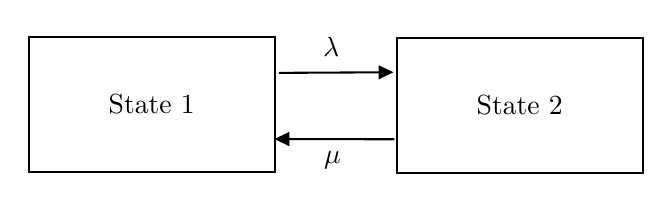
\begin{tikzpicture}[scale=0.8,x=0.75pt,y=0.75pt,yscale=-1,xscale=1]
%uncomment if require: \path (0,300); %set diagram left start at 0, and has height of 300

%Shape: Rectangle [id:dp6461073533685131] 
\draw   (20.57,59.47) -- (168.67,59.47) -- (168.67,140.67) -- (20.57,140.67) -- cycle ;
%Straight Lines [id:da9206552550981602] 
\draw    (171.25,81.07) -- (238.2,80.71) ;
\draw [shift={(240.2,80.7)}, rotate = 539.7] [fill={rgb, 255:red, 0; green, 0; blue, 0 }  ][line width=0.75]  [draw opacity=0] (8.93,-4.29) -- (0,0) -- (8.93,4.29) -- cycle    ;

%Straight Lines [id:da16336977884683224] 
\draw    (170.57,120.9) -- (240.75,121.07) ;

\draw [shift={(168.57,120.9)}, rotate = 0.13] [fill={rgb, 255:red, 0; green, 0; blue, 0 }  ][line width=0.75]  [draw opacity=0] (8.93,-4.29) -- (0,0) -- (8.93,4.29) -- cycle    ;
%Shape: Rectangle [id:dp6701645831587428] 
\draw   (242.23,59.97) -- (390.33,59.97) -- (390.33,141.17) -- (242.23,141.17) -- cycle ;

% Text Node
\draw (94.62,100.07) node  [align=left] {{\fontfamily{ptm}\selectfont State 1}};
% Text Node
\draw (316.28,100.57) node  [align=left] {{\fontfamily{ptm}\selectfont State 2}};
% Text Node
\draw (202.7,65.3) node   {$\lambda $};
% Text Node
\draw (203.8,133.6) node   {$\mu $};

\end{tikzpicture}
\end{center}
\end{frame}

\begin{frame}{Solution: Transition Rate Matrix}
\protect\phantomsection\label{solution-transition-rate-matrix}
The diagonal entries are the negatives of the total rates of leaving
each state.

\begin{itemize}
\tightlist
\item
  From State 1, the total rate of leaving is \(\lambda\), so
  \(q_{11}=-\lambda\).
\item
  From State 2, the total rate of leaving is \(\mu\), so
  \(q_{22}=-\mu\).
\end{itemize}

The off-diagonal entries are the transition rates shown in the diagram.
Hence,

\[
\boxed{
Q=
\begin{pmatrix}
-\lambda & \lambda\\
\mu & -\mu
\end{pmatrix}.
}
\]

Each row sums to zero, as required.
\end{frame}

\begin{frame}{Worked Example: Health-Sickness-Death Model}
\protect\phantomsection\label{worked-example-health-sickness-death-model}
Consider a time-homogeneous health-sickness-death (HSD) model with three
states:

\begin{itemize}
\tightlist
\item
  Healthy (\(h\));
\item
  Ill (\(i\));
\item
  Dead (\(d\)).
\end{itemize}

The transition rates are constant and are denoted by \(\sigma\),
\(\rho\), \(\mu\) and \(\nu\), as shown in the transition diagram.

Write down the transition rate matrix \(Q\).
\end{frame}

\begin{frame}{Solution: Transition Diagram}
\protect\phantomsection\label{solution-transition-diagram-1}
The transition diagram is

\begin{center}
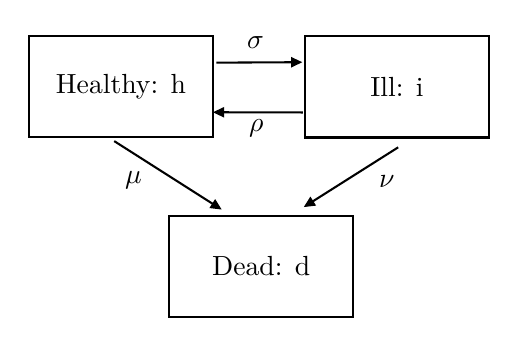
\begin{tikzpicture}[scale=0.6,x=0.75pt,y=0.75pt,yscale=-1,xscale=1]
%uncomment if require: \path (0,427); %set diagram left start at 0, and has height of 427

%Shape: Rectangle [id:dp6461073533685131] 
\draw   (20.57,59.47) -- (168.67,59.47) -- (168.67,140.67) -- (20.57,140.67) -- cycle ;
%Straight Lines [id:da9206552550981602] 
\draw    (171.25,81.07) -- (238.2,80.71) ;
\draw [shift={(240.2,80.7)}, rotate = 539.7] [fill={rgb, 255:red, 0; green, 0; blue, 0 }  ][line width=0.75]  [draw opacity=0] (8.93,-4.29) -- (0,0) -- (8.93,4.29) -- cycle    ;

%Straight Lines [id:da16336977884683224] 
\draw    (170.57,120.9) -- (240.75,121.07) ;

\draw [shift={(168.57,120.9)}, rotate = 0.13] [fill={rgb, 255:red, 0; green, 0; blue, 0 }  ][line width=0.75]  [draw opacity=0] (8.93,-4.29) -- (0,0) -- (8.93,4.29) -- cycle    ;
%Shape: Rectangle [id:dp6701645831587428] 
\draw   (242.23,59.97) -- (390.33,59.97) -- (390.33,141.17) -- (242.23,141.17) -- cycle ;
%Shape: Rectangle [id:dp5857755229985386] 
\draw   (133.23,203.97) -- (281.33,203.97) -- (281.33,285.17) -- (133.23,285.17) -- cycle ;
%Straight Lines [id:da26767212610765867] 
\draw    (89.25,144.07) -- (173.81,197.93) ;
\draw [shift={(175.5,199)}, rotate = 212.49] [fill={rgb, 255:red, 0; green, 0; blue, 0 }  ][line width=0.75]  [draw opacity=0] (8.93,-4.29) -- (0,0) -- (8.93,4.29) -- cycle    ;

%Straight Lines [id:da34728994666942503] 
\draw    (317.25,149.07) -- (243.19,195.93) ;
\draw [shift={(241.5,197)}, rotate = 327.68] [fill={rgb, 255:red, 0; green, 0; blue, 0 }  ][line width=0.75]  [draw opacity=0] (8.93,-4.29) -- (0,0) -- (8.93,4.29) -- cycle    ;


% Text Node
\draw (94.62,100.07) node  [align=left] {{\fontfamily{ptm}\selectfont Healthy: \textit{h}}};
% Text Node
\draw (202.7,65.3) node   {$\sigma $};
% Text Node
\draw (203.8,133.6) node   {$\rho $};
% Text Node
\draw (316.28,100.57) node  [align=left] {{\fontfamily{ptm}\selectfont Ill: \textit{i}}};
% Text Node
\draw (207.28,244.57) node  [align=left] {{\fontfamily{ptm}\selectfont Dead: \textit{d}}};
% Text Node
\draw (104.7,175.3) node   {$\mu $};
% Text Node
\draw (307.7,176.3) node   {$\nu $};


\end{tikzpicture}
\end{center}

The Dead state is absorbing: once the process enters this state, it
cannot leave.
\end{frame}

\begin{frame}{Solution: Transition Rate Matrix}
\protect\phantomsection\label{solution-transition-rate-matrix-1}
Using the state ordering \((h,i,d)\), the off-diagonal entries are
determined by the transition rates in the diagram.

The total rate of leaving each state is:

\begin{itemize}
\tightlist
\item
  Healthy: \(\sigma+\mu\);
\item
  Ill: \(\rho+\nu\);
\item
  Dead: \(0\).
\end{itemize}

Therefore, the diagonal entries are the negatives of these total rates.

The transition rate matrix is

\[
\boxed{
Q=
\begin{pmatrix}
-(\sigma+\mu) & \sigma & \mu\\
\rho & -(\rho+\nu) & \nu\\
0 & 0 & 0
\end{pmatrix}.
}
\]

Notice that every row sums to zero, and all off-diagonal entries are
non-negative.
\end{frame}

\begin{frame}{Worked Example: Generator Matrix of a Poisson Process}
\protect\phantomsection\label{worked-example-generator-matrix-of-a-poisson-process}
Consider a homogeneous Poisson process \(\{N(t)\}_{t\geq 0}\) with rate
\(\lambda>0\), where \(N(t)\) represents the number of events that have
occurred by time \(t\).

The process is a time-homogeneous Markov jump process with state space

\[
S=\{0,1,2,\ldots\}.
\]

\begin{enumerate}
\tightlist
\item
  Draw the state transition diagram.
\item
  Write down the transition rate matrix \(Q\).
\end{enumerate}
\end{frame}

\begin{frame}{Solution: State Transition Diagram}
\protect\phantomsection\label{solution-state-transition-diagram}
In a Poisson process, each event increases the number of events by
exactly one. Therefore, the only possible transition from state \(i\) is
to state \(i+1\), at rate \(\lambda\).

The transition diagram is

\begin{center}
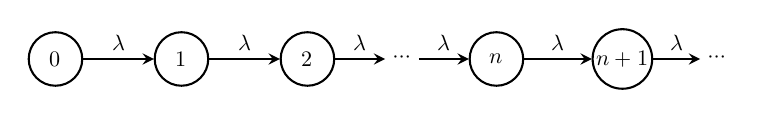
\begin{tikzpicture}[
  scale=0.8,
  transform shape,
  state/.style={
    draw,
    circle,
    minimum size=0.85cm,
    inner sep=1pt
  },
  transition/.style={->, >=stealth, thick}
]
\node[state] (S0) at (0,0) {$0$};
\node[state] (S1) at (2,0) {$1$};
\node[state] (S2) at (4,0) {$2$};
\node (dots1) at (5.5,0) {$\cdots$};
\node[state] (S3) at (7,0) {$n$};
\node[state] (S4) at (9,0) {$n+1$};
\node (dots2) at (10.5,0) {$\cdots$};

\draw[transition] (S0) -- node[above] {$\lambda$} (S1);
\draw[transition] (S1) -- node[above] {$\lambda$} (S2);
\draw[transition] (S2) -- node[above] {$\lambda$} (dots1);
\draw[transition] (dots1) -- node[above] {$\lambda$} (S3);
\draw[transition] (S3) -- node[above] {$\lambda$} (S4);
\draw[transition] (S4) -- node[above] {$\lambda$} (dots2);
\end{tikzpicture}
\end{center}
\end{frame}

\begin{frame}{Solution: Transition Rate Matrix}
\protect\phantomsection\label{solution-transition-rate-matrix-2}
The state space is countably infinite, so the generator matrix \(Q\) is
an infinite matrix.

From every state \(i\):

\begin{itemize}
\tightlist
\item
  The rate of moving to state \(i+1\) is \(\lambda\).
\item
  The total rate of leaving state \(i\) is \(\lambda\).
\item
  All other transition rates are zero.
\end{itemize}

Hence,

\[
\boxed{
Q=
\begin{pmatrix}
-\lambda & \lambda & 0 & 0 & 0 & \cdots\\
0 & -\lambda & \lambda & 0 & 0 & \cdots\\
0 & 0 & -\lambda & \lambda & 0 & \cdots\\
0 & 0 & 0 & -\lambda & \lambda & \cdots\\
\vdots & \vdots & \vdots & \ddots & \ddots & \ddots
\end{pmatrix}.
}
\]
\end{frame}

\begin{frame}{Solution: Transition Rate Matrix}
\protect\phantomsection\label{solution-transition-rate-matrix-3}
Equivalently, the entries of \(Q\) are

\[
q_{ij}=
\begin{cases}
-\lambda, & j=i,\\
\lambda, & j=i+1,\\
0, & \text{otherwise}.
\end{cases}
\]

Every row sums to zero, and all off-diagonal entries are non-negative.
\end{frame}

\section{Kolmogorov's Differential
Equations}\label{kolmogorovs-differential-equations}

\begin{frame}{From Transition Rates to Transition Probabilities}
\protect\phantomsection\label{from-transition-rates-to-transition-probabilities}
The generator matrix \(Q\) describes the instantaneous transition rates
of a Markov jump process.

However, in many practical applications, we are interested in
probabilities such as:

\begin{itemize}
\tightlist
\item
  The probability of being in a particular state after \(t\) years;
\item
  The probability of moving from one state to another over a specified
  period;
\item
  The probability distribution of the process at a future time.
\end{itemize}

Kolmogorov's differential equations provide the mathematical link
between the \textbf{transition rates} and the \textbf{transition
probabilities}.

Given the generator matrix \(Q\), these equations can be solved to
obtain the transition probability matrix \(P(t)\).
\end{frame}

\begin{frame}{Practical Importance of Kolmogorov's Equations}
\protect\phantomsection\label{practical-importance-of-kolmogorovs-equations}
In practice, the generator matrix is often estimated from observed data.

The general procedure is:

\begin{enumerate}
\tightlist
\item
  Collect data on the transitions between states and the time spent in
  each state.
\item
  Estimate the transition rates and construct the generator matrix
  \(Q\).
\item
  Use Kolmogorov's differential equations to determine the transition
  probability matrix \(P(t)\).
\item
  Use \(P(t)\) to calculate probabilities and make predictions about the
  future behaviour of the process.
\end{enumerate}

Thus, Kolmogorov's equations provide the link between statistical
estimation of transition rates and the calculation of transition
probabilities.
\end{frame}

\begin{frame}{Kolmogorov's Forward Differential Equations}
\protect\phantomsection\label{kolmogorovs-forward-differential-equations}
For a time-homogeneous Markov jump process, the forward differential
equations are

\[
\boxed{
\frac{d}{dt}p_{ij}(t)
=
\sum_{k\in S}p_{ik}(t)q_{kj},
\qquad i,j\in S.
}
\]

In matrix form,

\[
\boxed{
\frac{d}{dt}P(t)=P(t)Q.
}
\]

The initial condition is

\[
P(0)=I,
\]

where \(I\) is the identity matrix.
\end{frame}

\begin{frame}{Kolmogorov's Forward Differential Equations}
\protect\phantomsection\label{kolmogorovs-forward-differential-equations-1}
The forward equations describe how the transition probabilities change
over time, starting from a specified initial state.
\end{frame}

\begin{frame}{Assumptions Underlying the General Markov Model}
\protect\phantomsection\label{assumptions-underlying-the-general-markov-model}
Consider a time-homogeneous continuous-time Markov chain
\(\{X(t),t\geq 0\}\) with state space \(S\).

The model is based on the following assumptions.

\begin{enumerate}
\item
  \textbf{Markov assumption:} The future state depends on the current
  state, but not on the previous history of the process.
\item
  \textbf{Transition intensity:} For distinct states \(i\) and \(j\), \[
  \Pr(X(t+h)=j\mid X(t)=i)
  =\mu_{ij}h+o(h),
  \] where \(\mu_{ij}\) is the constant transition intensity from state
  \(i\) to state \(j\).
\item
  \textbf{Single-transition assumption:} The probability of two or more
  transitions during a short interval of length \(h\) is \(o(h)\).
\end{enumerate}

Here, \(h\downarrow 0\) and \(o(h)\) denotes a quantity whose ratio to
\(h\) tends to zero.
\end{frame}

\begin{frame}{Small-Time Transition Probabilities}
\protect\phantomsection\label{small-time-transition-probabilities}
The assumptions imply the following approximations for a small time
interval \(h\).

For distinct states \(i\) and \(j\),

\[
p_{ij}(h)=\mu_{ij}h+o(h).
\]

For the probability of remaining in state \(i\),

\[
p_{ii}(h)
=1-\sum_{j\neq i}\mu_{ij}h+o(h).
\]

Thus, the probability of leaving state \(i\) during a short interval is
approximately

\[
\left(\sum_{j\neq i}\mu_{ij}\right)h.
\]
\end{frame}

\begin{frame}{Small-Time Transition Probabilities}
\protect\phantomsection\label{small-time-transition-probabilities-1}
The total rate of leaving state \(i\) is

\[
\lambda_i=\sum_{j\neq i}\mu_{ij}=-q_{ii}.
\]

These approximations form the basis for deriving the Kolmogorov forward
equations.
\end{frame}

\begin{frame}{Derivation of the Kolmogorov Forward Equations}
\protect\phantomsection\label{derivation-of-the-kolmogorov-forward-equations}
We use the Chapman--Kolmogorov equation:

\[
p_{ij}(t+h)=\sum_{k\in S}p_{ik}(t)p_{kj}(h).
\]

For a small interval \(h\), the probability of being in state \(j\) at
time \(t+h\) has two main contributions:

\begin{itemize}
\tightlist
\item
  The process is already in state \(j\) at time \(t\) and remains there
  during the interval.
\item
  The process is in another state \(k\neq j\) at time \(t\) and moves to
  state \(j\) during the interval.
\end{itemize}

Using the small-time approximations,

\[
p_{ij}(t+h)=p_{ij}(t)\left(1-\sum_{\ell\neq j}\mu_{j\ell}h\right)+\sum_{k\neq j}p_{ik}(t)\mu_{kj}h+o(h).
\]
\end{frame}

\begin{frame}{Derivation of the Kolmogorov Forward Equations}
\protect\phantomsection\label{derivation-of-the-kolmogorov-forward-equations-1}
Subtracting \(p_{ij}(t)\), dividing by \(h\) and letting
\(h\downarrow 0\) gives

\[
\boxed{
p_{ij}'(t)
=
\sum_{k\neq j}p_{ik}(t)\mu_{kj}
-
p_{ij}(t)\sum_{\ell\neq j}\mu_{j\ell}.
}
\]

This is the Kolmogorov forward equation expressed in terms of transition
intensities.
\end{frame}

\begin{frame}{Interpretation of the Forward Equations}
\protect\phantomsection\label{interpretation-of-the-forward-equations}
The forward equation can be interpreted in terms of probability flow
into and out of state \(j\).

\[
\frac{d}{dt}p_{ij}(t)
=
\underbrace{\sum_{k\neq j}p_{ik}(t)\mu_{kj}}_{\text{Probability flow into state }j}
-
\underbrace{p_{ij}(t)\sum_{\ell\neq j}\mu_{j\ell}}_{\text{Probability flow out of state }j}.
\]

\begin{itemize}
\tightlist
\item
  \textbf{Inflow:} The process is in another state \(k\) at time \(t\)
  and moves to state \(j\).
\item
  \textbf{Outflow:} The process is in state \(j\) at time \(t\) and
  moves to another state.
\end{itemize}

The rate of change in the probability of occupying state \(j\) is the
total inflow minus the total outflow.
\end{frame}

\begin{frame}{Diagram Illustrating Probability Flow}
\protect\phantomsection\label{diagram-illustrating-probability-flow}
The following diagram illustrates the probability flow into state \(j\)
over a short time interval.

\begin{center}
\resizebox{0.8\textwidth}{!}{%
\tikzset{every picture/.style={line width=0.75pt}}
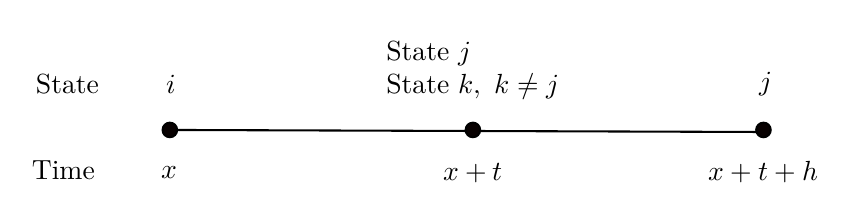
\begin{tikzpicture}[x=0.75pt,y=0.75pt,yscale=-1,xscale=1]
% Straight Lines
\draw (102,81.5) -- (391,82.5);

% State markers
\draw [fill={rgb,255:red,8;green,1;blue,1},fill opacity=1]
(98.5,81.5) .. controls (98.5,79.57) and (100.07,78) .. (102,78)
.. controls (103.93,78) and (105.5,79.57) .. (105.5,81.5)
.. controls (105.5,83.43) and (103.93,85) .. (102,85)
.. controls (100.07,85) and (98.5,83.43) .. (98.5,81.5) -- cycle;

\draw [fill={rgb,255:red,8;green,1;blue,1},fill opacity=1]
(244.5,81.5) .. controls (244.5,79.57) and (246.07,78) .. (248,78)
.. controls (249.93,78) and (251.5,79.57) .. (251.5,81.5)
.. controls (251.5,83.43) and (249.93,85) .. (248,85)
.. controls (246.07,85) and (244.5,83.43) .. (244.5,81.5) -- cycle;

\draw [fill={rgb,255:red,8;green,1;blue,1},fill opacity=1]
(384.5,81.5) .. controls (384.5,79.57) and (386.07,78) .. (388,78)
.. controls (389.93,78) and (391.5,79.57) .. (391.5,81.5)
.. controls (391.5,83.43) and (389.93,85) .. (388,85)
.. controls (386.07,85) and (384.5,83.43) .. (384.5,81.5) -- cycle;

% Text labels
\draw (102,102) node {$x$};
\draw (102.67,59.67) node {$i$};
\draw (34,95) node [anchor=north west][inner sep=0.75pt] {Time};
\draw (36,53) node [anchor=north west][inner sep=0.75pt] {State};
\draw (248,102) node {$x+t$};
\draw (247.67,52.67) node {$
\begin{array}{l}
\text{State }j\\
\text{State }k,\ k\neq j
\end{array}$};
\draw (388,102) node {$x+t+h$};
\draw (388.67,59.67) node {$j$};
\end{tikzpicture}%
}
\end{center}

At time \(t\), the process may be in state \(j\) or in another state
\(k\neq j\). During the short interval \(h\), probability flows into
state \(j\) from the other states and flows out of state \(j\) to other
states.
\end{frame}

\begin{frame}{Interpreting the Forward Equations}
\protect\phantomsection\label{interpreting-the-forward-equations}
Consider the probability of being in state \(j\) at time \(t\), given
that the process started in state \(i\).

The forward equation is

\[
p_{ij}'(t)=\sum_{k\in S}p_{ik}(t)q_{kj}.
\]

The equation considers all possible states \(k\) that the process may
occupy at time \(t\).

For each state \(k\):

\begin{itemize}
\tightlist
\item
  \(p_{ik}(t)\) is the probability of being in state \(k\) at time
  \(t\), starting from state \(i\).
\item
  \(q_{kj}\) is the instantaneous transition rate from state \(k\) to
  state \(j\).
\end{itemize}

The forward equations therefore describe how probability flows into each
destination state.
\end{frame}

\begin{frame}{Kolmogorov's Backward Differential Equations}
\protect\phantomsection\label{kolmogorovs-backward-differential-equations}
The transition probabilities also satisfy the \textbf{backward
differential equations}:

\[
\boxed{
\frac{d}{dt}p_{ij}(t)
=
\sum_{k\in S}q_{ik}p_{kj}(t),
\qquad i,j\in S.
}
\]

In matrix form,

\[
\boxed{
\frac{d}{dt}P(t)=QP(t).
}
\]

The initial condition is again \(P(0)=I.\)

The backward equations describe how the transition probabilities change
when we consider the possible first transitions from the initial state.
\end{frame}

\begin{frame}{Forward and Backward Equations: Comparison}
\protect\phantomsection\label{forward-and-backward-equations-comparison}
Both equations describe the evolution of the same transition probability
matrix, but they use the generator matrix in a different order.

{\def\LTcaptype{none} % do not increment counter
\begin{longtable}[]{@{}
  >{\raggedright\arraybackslash}p{(\linewidth - 2\tabcolsep) * \real{0.5000}}
  >{\raggedright\arraybackslash}p{(\linewidth - 2\tabcolsep) * \real{0.5000}}@{}}
\toprule\noalign{}
\begin{minipage}[b]{\linewidth}\raggedright
Forward equations
\end{minipage} & \begin{minipage}[b]{\linewidth}\raggedright
Backward equations
\end{minipage} \\
\midrule\noalign{}
\endhead
\(P'(t)=P(t)Q\) & \(P'(t)=QP(t)\) \\
Focus on the destination state & Focus on the initial state \\
Describe probability flow into destination states & Describe the effect
of possible first transitions \\
\bottomrule\noalign{}
\end{longtable}
}
\end{frame}

\begin{frame}{Forward and Backward Equations: Comparison}
\protect\phantomsection\label{forward-and-backward-equations-comparison-1}
For a finite-state, time-homogeneous Markov jump process, both equations
lead to

\[
\boxed{
P(t)=e^{Qt}.
}
\]

Thus, either set of equations can be used to determine the transition
probabilities.

The forward equations are often used to study the evolution of state
probabilities, while the backward equations are useful in problems
involving expected costs, rewards and times to reach specified states.
\end{frame}

\begin{frame}{Worked Example: A Two-State Markov Jump Process}
\protect\phantomsection\label{worked-example-a-two-state-markov-jump-process-1}
Consider a time-homogeneous Markov jump process with two states, State 0
and State 1. For example, these may represent a healthy individual and a
sick individual, respectively.

The transition rates are:

\begin{itemize}
\tightlist
\item
  \(\lambda\) from State 0 to State 1;
\item
  \(\mu\) from State 1 to State 0.
\end{itemize}

The generator matrix is

\[
Q=
\begin{pmatrix}
-\lambda & \lambda\\
\mu & -\mu
\end{pmatrix},
\qquad \lambda,\mu>0.
\]
\end{frame}

\begin{frame}{Worked Example: A Two-State Markov Jump Process}
\protect\phantomsection\label{worked-example-a-two-state-markov-jump-process-2}
\textbf{Questions} 1. Draw the state transition diagram. 2. Write down
the forward differential equations. 3. Verify that the following
expressions satisfy the forward differential equations:

\[
\begin{aligned}
p_{00}(t)
&=\frac{\mu}{\lambda+\mu}
+\frac{\lambda}{\lambda+\mu}
e^{-(\lambda+\mu)t},\\
p_{01}(t)
&=\frac{\lambda}{\lambda+\mu}
-\frac{\lambda}{\lambda+\mu}
e^{-(\lambda+\mu)t}.
\end{aligned}
\]

\begin{enumerate}
\setcounter{enumi}{3}
\tightlist
\item
  Obtain expressions for \(p_{10}(t)\) and \(p_{11}(t)\).
\item
  Find the limiting transition probability matrix as \(t\to\infty\) and
  interpret the result.
\end{enumerate}
\end{frame}

\begin{frame}{Solution: State Transition Diagram and Forward Equations}
\protect\phantomsection\label{solution-state-transition-diagram-and-forward-equations}
The transition diagram is

\begin{center}
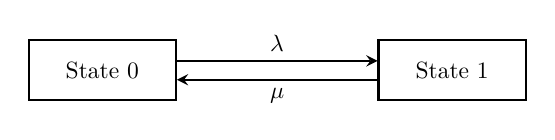
\begin{tikzpicture}[
  scale=0.85,
  transform shape,
  state/.style={
    draw,
    rectangle,
    minimum width=2.2cm,
    minimum height=0.9cm,
    align=center
  },
  transition/.style={->, >=stealth, thick}
]
\node[state] (S0) {State 0};
\node[state, right=3cm of S0] (S1) {State 1};

\draw[transition]
  ([yshift=4pt]S0.east) -- node[above] {$\lambda$} ([yshift=4pt]S1.west);

\draw[transition]
  ([yshift=-4pt]S1.west) -- node[below] {$\mu$} ([yshift=-4pt]S0.east);
\end{tikzpicture}
\end{center}

The forward equations are obtained from

\[
P'(t)=P(t)Q.
\]

For each initial state \(i\in\{0,1\}\),

\[
\begin{aligned}
p_{i0}'(t)
&=-\lambda p_{i0}(t)+\mu p_{i1}(t),\\
p_{i1}'(t)
&=\lambda p_{i0}(t)-\mu p_{i1}(t).
\end{aligned}
\]
\end{frame}

\begin{frame}{Solution: State Transition Diagram and Forward Equations}
\protect\phantomsection\label{solution-state-transition-diagram-and-forward-equations-1}
The initial conditions are

\[
p_{ij}(0)=
\begin{cases}
1, & i=j,\\
0, & i\neq j.
\end{cases}
\]
\end{frame}

\begin{frame}{Solution: Transition Probabilities from State 0}
\protect\phantomsection\label{solution-transition-probabilities-from-state-0}
Starting from State 0, the initial conditions are

\[
p_{00}(0)=1,
\qquad
p_{01}(0)=0.
\]

The forward equations become

\[
\begin{aligned}
p_{00}'(t)
&=-\lambda p_{00}(t)+\mu p_{01}(t),\\
p_{01}'(t)
&=\lambda p_{00}(t)-\mu p_{01}(t).
\end{aligned}
\]

Since the probabilities in each row sum to one,

\[
p_{00}(t)+p_{01}(t)=1.
\]
\end{frame}

\begin{frame}{Solution: Transition Probabilities from State 0}
\protect\phantomsection\label{solution-transition-probabilities-from-state-0-1}
Substituting \(p_{00}(t)=1-p_{01}(t)\) into the second equation gives

\[
p_{01}'(t)
=
\lambda-(\lambda+\mu)p_{01}(t).
\]

Solving this differential equation with \(p_{01}(0)=0\) gives

\[
\boxed{
p_{01}(t)
=
\frac{\lambda}{\lambda+\mu}
\left(1-e^{-(\lambda+\mu)t}\right).
}
\]

Consequently,

\[
\boxed{
p_{00}(t)
=
\frac{\mu}{\lambda+\mu}
+
\frac{\lambda}{\lambda+\mu}
e^{-(\lambda+\mu)t}.
}
\]
\end{frame}

\begin{frame}{Solution: Transition Probabilities from State 1}
\protect\phantomsection\label{solution-transition-probabilities-from-state-1}
Starting from State 1, the initial conditions are

\[
p_{10}(0)=0,
\qquad
p_{11}(0)=1.
\]

Using the forward equations and the condition

\[
p_{10}(t)+p_{11}(t)=1,
\]

we obtain

\[
p_{10}'(t)
=
\mu-(\lambda+\mu)p_{10}(t).
\]
\end{frame}

\begin{frame}{Solution: Transition Probabilities from State 1}
\protect\phantomsection\label{solution-transition-probabilities-from-state-1-1}
Solving this differential equation gives

\[
\boxed{
p_{10}(t)
=
\frac{\mu}{\lambda+\mu}
\left(1-e^{-(\lambda+\mu)t}\right).
}
\]

Therefore,

\[
\boxed{
p_{11}(t)
=
\frac{\lambda}{\lambda+\mu}
+
\frac{\mu}{\lambda+\mu}
e^{-(\lambda+\mu)t}.
}
\]
\end{frame}

\begin{frame}{Solution: Transition Probability Matrix}
\protect\phantomsection\label{solution-transition-probability-matrix}
Combining the four transition probabilities gives

\[
\boxed{
P(t)=
\begin{pmatrix}
\displaystyle
\frac{\mu+\lambda e^{-(\lambda+\mu)t}}
{\lambda+\mu}
&
\displaystyle
\frac{\lambda(1-e^{-(\lambda+\mu)t})}
{\lambda+\mu}
\\[12pt]
\displaystyle
\frac{\mu(1-e^{-(\lambda+\mu)t})}
{\lambda+\mu}
&
\displaystyle
\frac{\lambda+\mu e^{-(\lambda+\mu)t}}
{\lambda+\mu}
\end{pmatrix}.
}
\]

Notice that each row sums to one, and \(P(0)=I\).
\end{frame}

\begin{frame}{Solution: Limiting Transition Probability Matrix}
\protect\phantomsection\label{solution-limiting-transition-probability-matrix}
As \(t\to\infty\),

\[
e^{-(\lambda+\mu)t}\longrightarrow 0.
\]

Hence,

\[
\boxed{
\lim_{t\to\infty}P(t)
=
\begin{pmatrix}
\displaystyle\frac{\mu}{\lambda+\mu}
&
\displaystyle\frac{\lambda}{\lambda+\mu}
\\[8pt]
\displaystyle\frac{\mu}{\lambda+\mu}
&
\displaystyle\frac{\lambda}{\lambda+\mu}
\end{pmatrix}.
}
\]
\end{frame}

\begin{frame}{Solution: Limiting Transition Probability Matrix}
\protect\phantomsection\label{solution-limiting-transition-probability-matrix-1}
The limiting distribution is

\[
\boldsymbol{\pi}
=
\left(
\frac{\mu}{\lambda+\mu},
\frac{\lambda}{\lambda+\mu}
\right).
\]

Both rows of the limiting matrix are identical. Therefore, the limiting
distribution does not depend on the initial state.

In the long run, the process spends a proportion \(\mu/(\lambda+\mu)\)
of its time in State 0 and a proportion \(\lambda/(\lambda+\mu)\) of its
time in State 1.
\end{frame}

\begin{frame}{Why the Backward Equations Are Useful}
\protect\phantomsection\label{why-the-backward-equations-are-useful}
The forward equations describe how probabilities evolve from a given
initial state.

The backward equations are useful when we want to study how the initial
state affects a future quantity.

For example, let \(g(j)\) be a cost or reward associated with being in
state \(j\) at time \(t\). Define

\[
u_i(t)
=
\sum_{j\in S}p_{ij}(t)g(j).
\]

This is the expected cost or reward at time \(t\), given that the
process starts in state \(i\).

Using the backward equations, we obtain

\[
\boxed{
\frac{d}{dt}u_i(t)
=
\sum_{k\in S}q_{ik}u_k(t).
}
\]
\end{frame}

\begin{frame}{Why the Backward Equations Are Useful}
\protect\phantomsection\label{why-the-backward-equations-are-useful-1}
Thus, the backward equations can be used to study expected future costs
and rewards from different initial states.

They are also useful in calculating expected times to reach a specified
state, which we will consider later in this chapter.
\end{frame}

\begin{frame}{Interpretation of the Transition Probability
\(p_{ii}(t)\)}
\protect\phantomsection\label{interpretation-of-the-transition-probability-p_iit}
It is important to distinguish between two different probabilities.

The transition probability

\[
p_{ii}(t)
=
\Pr(X(s+t)=i\mid X(s)=i)
\]

is the probability that the process is in state \(i\) at time \(s+t\),
given that it was in state \(i\) at time \(s\).

It does \textbf{not} require the process to remain in state \(i\)
throughout the interval \([s,s+t]\). The process may leave state \(i\)
and return before time \(s+t\).

In contrast, the probability of remaining continuously in state \(i\)
throughout the interval is

\[
\overline p_{ii}(t)
=
\Pr\bigl(X(u)=i\text{ for all }u\in[s,s+t]
\mid X(s)=i\bigr).
\]
\end{frame}

\begin{frame}{Interpretation of the Transition Probability
\(p_{ii}(t)\)}
\protect\phantomsection\label{interpretation-of-the-transition-probability-p_iit-1}
For a time-homogeneous Markov jump process, this probability is

\[
\boxed{
\overline p_{ii}(t)=e^{-(-q_{ii})t}.
}
\]

Here, \(-q_{ii}\) is the total rate of leaving state \(i\).

In the two-state model, for example,

\[
\overline p_{00}(t)=e^{-\lambda t},
\qquad
\overline p_{11}(t)=e^{-\mu t}.
\]

These are the survival probabilities of the holding times in States 0
and 1, respectively.
\end{frame}

\begin{frame}{Worked Example: A Terminal Illness Model}
\protect\phantomsection\label{worked-example-a-terminal-illness-model}
Consider a three-state Markov jump process representing the health
status of an individual:

\begin{itemize}
\tightlist
\item
  Well (\(w\));
\item
  Ill (\(i\));
\item
  Dead (\(d\)).
\end{itemize}

The transition diagram is shown below. The transition rates are
\(\sigma\) from Well to Ill and \(\mu\) from Ill to Dead. Assume that
both rates are constant.

\begin{enumerate}
\tightlist
\item
  Explain why \(p_{ww}(t)=\overline p_{ww}(t)\).
\item
  Explain why \(p_{ii}(t)=\overline p_{ii}(t)\).
\end{enumerate}
\end{frame}

\begin{frame}{Solution: Interpretation of Transition Probabilities}
\protect\phantomsection\label{solution-interpretation-of-transition-probabilities}
The transition diagram is

\begin{center}
\resizebox{0.85\textwidth}{!}{%
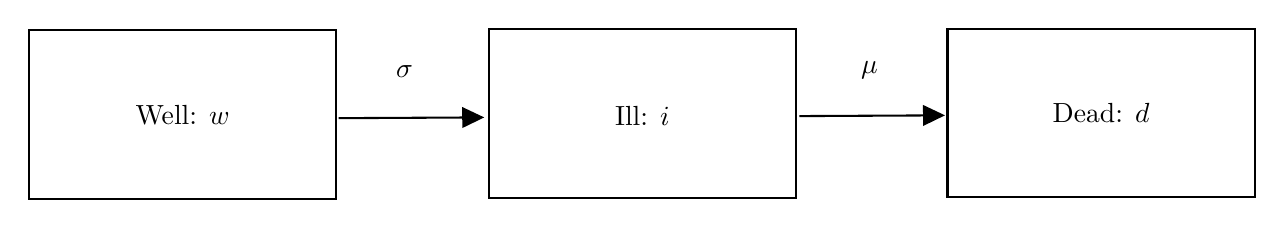
\begin{tikzpicture}[x=0.75pt,y=0.75pt,yscale=-1,xscale=1]
\draw (20.57,59.47) -- (168.67,59.47) -- (168.67,140.67) -- (20.57,140.67) -- cycle;
\draw (169.92,101.73) -- (236.87,101.38);
\draw [shift={(238.87,101.37)}, rotate=539.7] [fill=black] (8.93,-4.29) -- (0,0) -- (8.93,4.29) -- cycle;
\draw (242.23,58.97) -- (390.33,58.97) -- (390.33,140.17) -- (242.23,140.17) -- cycle;
\draw (463.23,58.63) -- (611.33,58.63) -- (611.33,139.83) -- (463.23,139.83) -- cycle;
\draw (391.92,100.73) -- (458.87,100.38);
\draw [shift={(460.87,100.37)}, rotate=539.7] [fill=black] (8.93,-4.29) -- (0,0) -- (8.93,4.29) -- cycle;
\draw (94.62,100.07) node [align=left] {{\fontfamily{ptm}\selectfont Well: $w$}};
\draw (201.37,79.3) node {$\sigma$};
\draw (316.28,100.57) node [align=left] {{\fontfamily{ptm}\selectfont Ill: $i$}};
\draw (537.28,99.23) node [align=left] {{\fontfamily{ptm}\selectfont Dead: $d$}};
\draw (426.03,78.63) node {$\mu$};
\end{tikzpicture}%
}
\end{center}

Since a transition from Ill to Well is impossible, once the process
leaves the Well state, it cannot return.

Therefore, being in the Well state at time \(s+t\) is equivalent to
having remained continuously in the Well state throughout the interval
\([s,s+t]\).

Hence,

\[
\boxed{
p_{ww}(t)=\overline p_{ww}(t).
}
\]
\end{frame}

\begin{frame}{Solution: Interpretation of Transition Probabilities}
\protect\phantomsection\label{solution-interpretation-of-transition-probabilities-1}
Similarly, once the process leaves the Ill state, it moves to the
absorbing Dead state and cannot return to Ill. Thus,

\[
\boxed{
p_{ii}(t)=\overline p_{ii}(t).
}
\]
\end{frame}

\begin{frame}{Worked Example: Working, Retiring and Dying}
\protect\phantomsection\label{worked-example-working-retiring-and-dying}
Consider a time-homogeneous three-state Markov jump model for an
individual's working life. The possible states are:

\begin{itemize}
\tightlist
\item
  Working (\(w\));
\item
  Retired (\(r\));
\item
  Dead (\(d\)).
\end{itemize}

Assume that the transition rates are constant. An individual can move
from Working to Retired at rate \(\nu\), or from Working to Dead at rate
\(\mu\). Both Retired and Dead are absorbing states.
\end{frame}

\begin{frame}{Worked Example: Working, Retiring and Dying}
\protect\phantomsection\label{worked-example-working-retiring-and-dying-1}
Answer the following questions:

\begin{enumerate}
\tightlist
\item
  What can you say about \(p_{ww}(t)\) and \(\overline p_{ww}(t)\)?
\item
  Write down the forward differential equations for \(p_{wd}(t)\),
  \(p_{wr}(t)\) and \(p_{ww}(t)\).
\item
  Solve the forward differential equation for \(p_{ww}(t)\).
\item
  Show that
\end{enumerate}

\[
\begin{aligned}
p_{wd}(t)
&=\frac{\mu}{\mu+\nu}
\left(1-e^{-(\mu+\nu)t}\right),\\
p_{wr}(t)
&=\frac{\nu}{\mu+\nu}
\left(1-e^{-(\mu+\nu)t}\right).
\end{aligned}
\]

\begin{enumerate}
\setcounter{enumi}{4}
\tightlist
\item
  Verify that
\end{enumerate}

\[
p_{wd}(t)+p_{wr}(t)+p_{ww}(t)=1.
\]
\end{frame}

\begin{frame}{Solution: Transition Diagram and Interpretation}
\protect\phantomsection\label{solution-transition-diagram-and-interpretation}
The transition diagram is

\begin{center}
\resizebox{0.65\textwidth}{!}{%
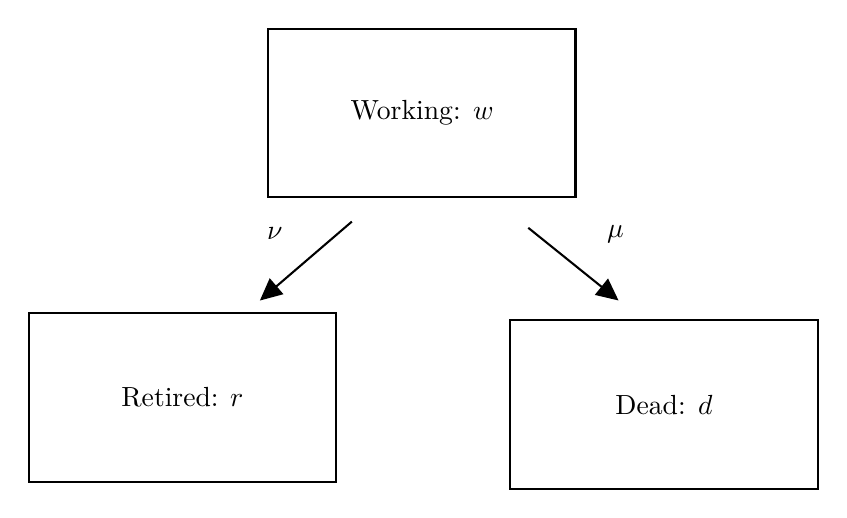
\begin{tikzpicture}[x=0.75pt,y=0.75pt,yscale=-1,xscale=1]
\draw (201.57,60.47) -- (349.67,60.47) -- (349.67,141.67) -- (201.57,141.67) -- cycle;
\draw (241.92,153.4) -- (200.02,189.36);
\draw [shift={(198.5,190.67)}, rotate=319.36] [fill=black] (8.93,-4.29) -- (0,0) -- (8.93,4.29) -- cycle;
\draw (318.23,200.97) -- (466.33,200.97) -- (466.33,282.17) -- (318.23,282.17) -- cycle;
\draw (86.23,197.63) -- (234.33,197.63) -- (234.33,278.83) -- (86.23,278.83) -- cycle;
\draw (326.92,156.4) -- (367.94,189.41);
\draw [shift={(369.5,190.67)}, rotate=218.82] [fill=black] (8.93,-4.29) -- (0,0) -- (8.93,4.29) -- cycle;
\draw (275.62,101.07) node [align=left] {{\fontfamily{ptm}\selectfont Working: $w$}};
\draw (204.37,159.3) node {$\nu$};
\draw (160.28,238.23) node [align=left] {{\fontfamily{ptm}\selectfont Retired: $r$}};
\draw (392.28,241.57) node [align=left] {{\fontfamily{ptm}\selectfont Dead: $d$}};
\draw (369.03,159.63) node {$\mu$};
\end{tikzpicture}%
}
\end{center}
\end{frame}

\begin{frame}{Solution: Transition Diagram and Interpretation}
\protect\phantomsection\label{solution-transition-diagram-and-interpretation-1}
Since returning to the Working state is impossible, the probability of
being in the Working state at time \(t\) is equal to the probability of
remaining continuously in that state.

Therefore,

\[
\boxed{
p_{ww}(t)=\overline p_{ww}(t).
}
\]
\end{frame}

\begin{frame}{Solution: Forward Differential Equations}
\protect\phantomsection\label{solution-forward-differential-equations}
Using the state ordering \((w,r,d)\), the transition rate matrix is

\[
Q=
\begin{pmatrix}
-(\nu+\mu) & \nu & \mu\\
0 & 0 & 0\\
0 & 0 & 0
\end{pmatrix}.
\]

The forward equations are obtained from

\[
P'(t)=P(t)Q.
\]

Starting from the Working state, the relevant equations are

\[
\begin{aligned}
p_{ww}'(t)
&=-(\nu+\mu)p_{ww}(t),\\
p_{wr}'(t)
&=\nu p_{ww}(t),\\
p_{wd}'(t)
&=\mu p_{ww}(t).
\end{aligned}
\]
\end{frame}

\begin{frame}{Solution: Forward Differential Equations}
\protect\phantomsection\label{solution-forward-differential-equations-1}
The initial conditions are

\[
p_{ww}(0)=1,
\qquad
p_{wr}(0)=p_{wd}(0)=0.
\]
\end{frame}

\begin{frame}{Solution: Probability of Remaining Working}
\protect\phantomsection\label{solution-probability-of-remaining-working}
The differential equation for \(p_{ww}(t)\) is

\[
p_{ww}'(t)=-(\nu+\mu)p_{ww}(t).
\]

Solving this equation with \(p_{ww}(0)=1\) gives

\[
\boxed{
p_{ww}(t)=e^{-(\nu+\mu)t}.
}
\]

Since \(p_{ww}(t)=\overline p_{ww}(t)\), this is also the probability of
remaining continuously in the Working state throughout the interval.
\end{frame}

\begin{frame}{Solution: Probabilities of Retirement and Death}
\protect\phantomsection\label{solution-probabilities-of-retirement-and-death}
From the forward equation for \(p_{wd}(t)\),

\[
p_{wd}'(t)=\mu e^{-(\nu+\mu)t}.
\]

Integrating from \(0\) to \(t\), and using \(p_{wd}(0)=0\), gives

\[
\begin{aligned}
p_{wd}(t)
&=\int_0^t\mu e^{-(\nu+\mu)s}\,ds\\
&=\boxed{
\frac{\mu}{\mu+\nu}
\left(1-e^{-(\mu+\nu)t}\right).
}
\end{aligned}
\]

Similarly,

\[
p_{wr}'(t)=\nu e^{-(\nu+\mu)t}.
\]
\end{frame}

\begin{frame}{Solution: Probabilities of Retirement and Death}
\protect\phantomsection\label{solution-probabilities-of-retirement-and-death-1}
Integrating and using \(p_{wr}(0)=0\) gives

\[
\boxed{
p_{wr}(t)
=
\frac{\nu}{\mu+\nu}
\left(1-e^{-(\mu+\nu)t}\right).
}
\]
\end{frame}

\begin{frame}{Solution: Verification of the Total Probability}
\protect\phantomsection\label{solution-verification-of-the-total-probability}
Adding the three transition probabilities gives

\[
\begin{aligned}
&p_{ww}(t)+p_{wr}(t)+p_{wd}(t)\\
&=e^{-(\mu+\nu)t}\\
&\quad+\frac{\nu}{\mu+\nu}
\left(1-e^{-(\mu+\nu)t}\right)\\
&\quad+\frac{\mu}{\mu+\nu}
\left(1-e^{-(\mu+\nu)t}\right)\\
&=e^{-(\mu+\nu)t}
+1-e^{-(\mu+\nu)t}\\
&=\boxed{1}.
\end{aligned}
\]

This is consistent with the fact that an individual starting in the
Working state must be in exactly one of the three states at time \(t\).
\end{frame}

\begin{frame}{Worked Example: Permanent Health Insurance (PHI) Model}
\protect\phantomsection\label{worked-example-permanent-health-insurance-phi-model}
Consider a three-state model for permanent health insurance (PHI). This
type of insurance provides a regular income to an individual who becomes
unable to work because of long-term illness or injury.

The possible states are:

\begin{itemize}
\tightlist
\item
  Healthy (\(h\));
\item
  Ill (\(i\));
\item
  Dead (\(d\)).
\end{itemize}

Assume that the transition diagram is the same as the
health-sickness-death model, with constant transition rates \(\sigma\),
\(\rho\), \(\mu\) and \(\nu\).

\begin{enumerate}
\tightlist
\item
  Write down the forward differential equations for \(p_{hh}(t)\),
  \(p_{hi}(t)\) and \(p_{hd}(t)\).
\item
  The equations for \(p_{hh}(t)\) and \(p_{hi}(t)\) can be solved
  simultaneously. Let
\end{enumerate}

\[
u(t)=p_{hi}(t),
\qquad
w(t)=p_{hh}(t).
\]

Show that \(u(t)\) satisfies the second-order linear differential
equation

\[
\boxed{
\frac{d^2u}{dt^2}
+(\sigma+\mu+\rho+\nu)\frac{du}{dt}
+(\sigma\nu+\mu\rho+\mu\nu)u=0.
}
\]
\end{frame}

\begin{frame}{Solution: Transition Diagram and Generator Matrix}
\protect\phantomsection\label{solution-transition-diagram-and-generator-matrix}
We assume that the transition diagram is the same as the
health-sickness-death model:

\begin{center}
\resizebox{0.65\textwidth}{!}{%
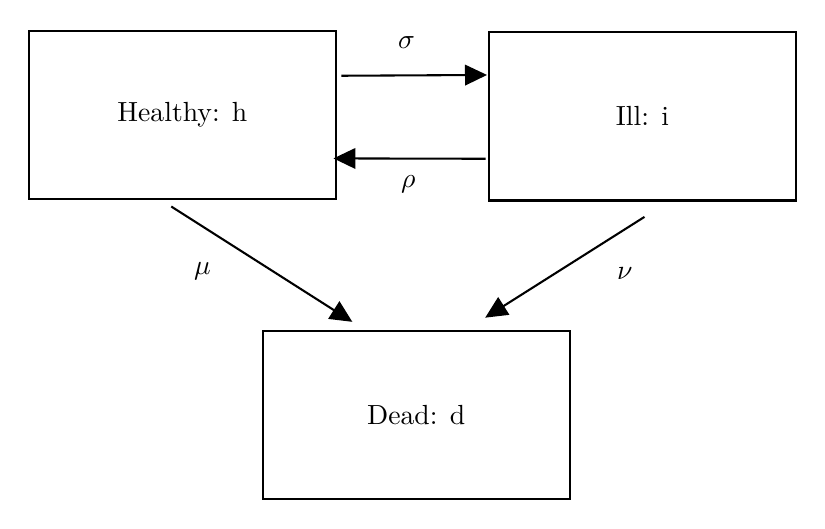
\begin{tikzpicture}[x=0.75pt,y=0.75pt,yscale=-1,xscale=1]
\draw (20.57,59.47) -- (168.67,59.47) -- (168.67,140.67) -- (20.57,140.67) -- cycle;
\draw (171.25,81.07) -- (238.2,80.71);
\draw [shift={(240.2,80.7)}, rotate=539.7] [fill=black] (8.93,-4.29) -- (0,0) -- (8.93,4.29) -- cycle;
\draw (170.57,120.9) -- (240.75,121.07);
\draw [shift={(168.57,120.9)}, rotate=0.13] [fill=black] (8.93,-4.29) -- (0,0) -- (8.93,4.29) -- cycle;
\draw (242.23,59.97) -- (390.33,59.97) -- (390.33,141.17) -- (242.23,141.17) -- cycle;
\draw (133.23,203.97) -- (281.33,203.97) -- (281.33,285.17) -- (133.23,285.17) -- cycle;
\draw (89.25,144.07) -- (173.81,197.93);
\draw [shift={(175.5,199)}, rotate=212.49] [fill=black] (8.93,-4.29) -- (0,0) -- (8.93,4.29) -- cycle;
\draw (317.25,149.07) -- (243.19,195.93);
\draw [shift={(241.5,197)}, rotate=327.68] [fill=black] (8.93,-4.29) -- (0,0) -- (8.93,4.29) -- cycle;
\draw (94.62,100.07) node [align=left] {{\fontfamily{ptm}\selectfont Healthy: \textit{h}}};
\draw (202.7,65.3) node {$\sigma$};
\draw (203.8,133.6) node {$\rho$};
\draw (316.28,100.57) node [align=left] {{\fontfamily{ptm}\selectfont Ill: \textit{i}}};
\draw (207.28,244.57) node [align=left] {{\fontfamily{ptm}\selectfont Dead: \textit{d}}};
\draw (104.7,175.3) node {$\mu$};
\draw (307.7,176.3) node {$\nu$};
\end{tikzpicture}%
}
\end{center}

Using the state ordering \((h,i,d)\), the transition rate matrix is

\[
Q=
\begin{pmatrix}
-(\sigma+\mu) & \sigma & \mu\\
\rho & -(\rho+\nu) & \nu\\
0 & 0 & 0
\end{pmatrix}.
\]
\end{frame}

\begin{frame}{Solution: Forward Differential Equations}
\protect\phantomsection\label{solution-forward-differential-equations-2}
The forward equations are obtained from

\[
P'(t)=P(t)Q.
\]

Starting from the Healthy state, we obtain

\[
\begin{aligned}
p_{hh}'(t)
&=-(\sigma+\mu)p_{hh}(t)
+\rho p_{hi}(t),\\
p_{hi}'(t)
&=\sigma p_{hh}(t)
-(\rho+\nu)p_{hi}(t),\\
p_{hd}'(t)
&=\mu p_{hh}(t)+\nu p_{hi}(t).
\end{aligned}
\]

The initial conditions are

\[
p_{hh}(0)=1,
\qquad
p_{hi}(0)=p_{hd}(0)=0.
\]
\end{frame}

\begin{frame}{Solution: Deriving the Second-Order Differential Equation}
\protect\phantomsection\label{solution-deriving-the-second-order-differential-equation}
Let

\[
u(t)=p_{hi}(t),
\qquad
w(t)=p_{hh}(t).
\]

The first two forward equations become

\[
\begin{aligned}
w'(t)
&=-(\sigma+\mu)w(t)+\rho u(t),\\
u'(t)
&=\sigma w(t)-(\rho+\nu)u(t).
\end{aligned}
\]

Rearranging the second equation gives

\[
w(t)=\frac{1}{\sigma}
\left\{u'(t)+(\rho+\nu)u(t)\right\}.
\]
\end{frame}

\begin{frame}{Solution: Deriving the Second-Order Differential Equation}
\protect\phantomsection\label{solution-deriving-the-second-order-differential-equation-1}
Differentiating the equation for \(u(t)\) gives

\[
u''(t)=\sigma w'(t)-(\rho+\nu)u'(t).
\]

Substituting the expression for \(w'(t)\),

\[
u''(t)
=
\sigma\left\{-(\sigma+\mu)w(t)+\rho u(t)\right\}
-(\rho+\nu)u'(t).
\]

Now substitute

\[
w(t)=\frac{u'(t)+(\rho+\nu)u(t)}{\sigma}.
\]
\end{frame}

\begin{frame}{Solution: Deriving the Second-Order Differential Equation}
\protect\phantomsection\label{solution-deriving-the-second-order-differential-equation-2}
After collecting terms, we obtain

\[
\begin{aligned}
u''(t)
&=-(\sigma+\mu)u'(t)\\
&\quad-(\sigma+\mu)(\rho+\nu)u(t)
+\sigma\rho u(t)\\
&\quad-(\rho+\nu)u'(t).
\end{aligned}
\]

Rearranging gives

\[
\boxed{
u''(t)
+(\sigma+\mu+\rho+\nu)u'(t)
+(\sigma\nu+\mu\rho+\mu\nu)u(t)=0.
}
\]

The initial conditions for this second-order equation follow from the
original forward equations:

\[
u(0)=0,
\qquad
u'(0)=\sigma.
\]
\end{frame}

\section{Holding Times and Occupancy
Probabilities}\label{holding-times-and-occupancy-probabilities}

\begin{frame}{Holding Times in a Markov Jump Process}
\protect\phantomsection\label{holding-times-in-a-markov-jump-process}
A Poisson process moves from state \(i\) to state \(i+1\) at each event.
In a general Markov jump process, however, the process can move from its
current state to any other state connected to it by a possible
transition.

The timing of these transitions has a feature in common with the Poisson
process: \textbf{the holding time in a given state is exponentially
distributed}.

However, unlike the Poisson process, the parameter of the exponential
distribution generally depends on the current state.

Let \(T_0\) denote the first holding time:

\[
T_0=\inf\{t>0:X(t)\neq X(0)\}.
\]

Thus, \(T_0\) is the time until the process first leaves its initial
state.
\end{frame}

\begin{frame}{Distribution of the First Holding Time}
\protect\phantomsection\label{distribution-of-the-first-holding-time}
Suppose the process starts in state \(i\). The total transition rate out
of state \(i\) is

\[
\lambda_i=\sum_{j\neq i}q_{ij}=-q_{ii}.
\]

\textbf{Theorem:} Conditional on \(X(0)=i\), the first holding time
\(T_0\) has an exponential distribution with parameter \(\lambda_i\).

In particular,
\(\boxed{\Pr(T_0>t\mid X(0)=i)=e^{-\lambda_i t}=e^{q_{ii}t},\qquad t\geq 0.}\)

If \(\lambda_i>0\), the corresponding density is

\[
f_{T_0\mid X(0)=i}(t)
=\lambda_i e^{-\lambda_i t},
\qquad t\geq 0.
\]

If \(\lambda_i=0\), state \(i\) is absorbing and the process never
leaves it.
\end{frame}

\begin{frame}{Interpreting the Holding-Time Distribution}
\protect\phantomsection\label{interpreting-the-holding-time-distribution}
The parameter \(\lambda_i\) is the \textbf{total rate of leaving state
\(i\)}. It is obtained by adding the rates of all possible transitions
out of that state.

The probability of remaining in state \(i\) for at least \(t\) time
units is

\[
\boxed{
\overline p_{ii}(t)
=\Pr(T_0>t\mid X(0)=i)
=e^{-\lambda_i t}.
}
\]

\textbf{We use an overline to denote this special probability, writing
it as \(\overline{p}_{ii}(t)\). This is the probability that the process
remains in state \(i\) throughout the entire interval \([0,t]\)}.

The expected holding time in state \(i\) is

\[
\boxed{
\operatorname{E}[T_0\mid X(0)=i]
=\frac{1}{\lambda_i}
=\frac{1}{-q_{ii}}.
}
\]

A larger total transition rate means a shorter expected holding time.
\end{frame}

\begin{frame}{Holding Times and the Poisson Process}
\protect\phantomsection\label{holding-times-and-the-poisson-process}
The holding time in state \(i\) has the memoryless property of the
exponential distribution.

For \(s,t\geq 0\),

\[
\Pr(T_0>s+t\mid T_0>s,\ X(0)=i)
=
\Pr(T_0>t\mid X(0)=i).
\]

Thus, conditional on still being in state \(i\), the remaining time
until the next transition has the same exponential distribution as the
original holding time.

This is similar to the inter-arrival times of a Poisson process. The
difference is that the rate of leaving a state in a general Markov jump
process depends on the state currently occupied.
\end{frame}

\begin{frame}{Continuous Occupancy and Transition Probabilities}
\protect\phantomsection\label{continuous-occupancy-and-transition-probabilities}
Two probabilities concerning state \(i\) must be distinguished.

\textbf{Continuous occupancy probability}

\[
\overline p_{ii}(t)
=
\Pr(X(s)=i\text{ for all }0\leq s\leq t\mid X(0)=i).
\]

This is the probability that the process remains in state \(i\)
throughout the entire interval \([0,t]\).

\textbf{Transition probability}

\[
p_{ii}(t)
=
\Pr(X(t)=i\mid X(0)=i).
\]

This is the probability that the process is in state \(i\) at time
\(t\). The process may have left state \(i\) and subsequently returned.
\end{frame}

\begin{frame}{Continuous Occupancy and Transition Probabilities}
\protect\phantomsection\label{continuous-occupancy-and-transition-probabilities-1}
Consequently,

\[
\boxed{
\overline p_{ii}(t)\leq p_{ii}(t).
}
\]

Equality holds when the process cannot return to state \(i\) after
leaving it.

For example, this equality holds in a model where state \(i\) can only
lead to absorbing states.
\end{frame}

\begin{frame}{Worked Example: A Four-State Health Model}
\protect\phantomsection\label{worked-example-a-four-state-health-model}
Consider a Health--Sickness--Terminally Ill--Death model with the
following four states:

\begin{itemize}
\tightlist
\item
  Healthy (H)
\item
  Sick (S)
\item
  Terminally Ill (T)
\item
  Dead (D), an absorbing state
\end{itemize}

The transition intensities are expressed on a yearly basis.

The transition-rate diagram or table specifies the possible transitions
and their corresponding intensities.

\textbf{Questions}

\begin{enumerate}
\tightlist
\item
  Write down the generator matrix \(Q\) for this four-state
  continuous-time Markov model.
\item
  Calculate the expected holding time in state H.
\end{enumerate}
\end{frame}

\begin{frame}{Worked Example: A Four-State Health Model}
\protect\phantomsection\label{worked-example-a-four-state-health-model-1}
The transition diagram of the Health--Sickness--Terminally Ill--Death
(H--S--T--D) multi-state model.

\tikzset{every picture/.style={line width=0.75pt}} %set default line width to 0.75pt        

\begin{center}
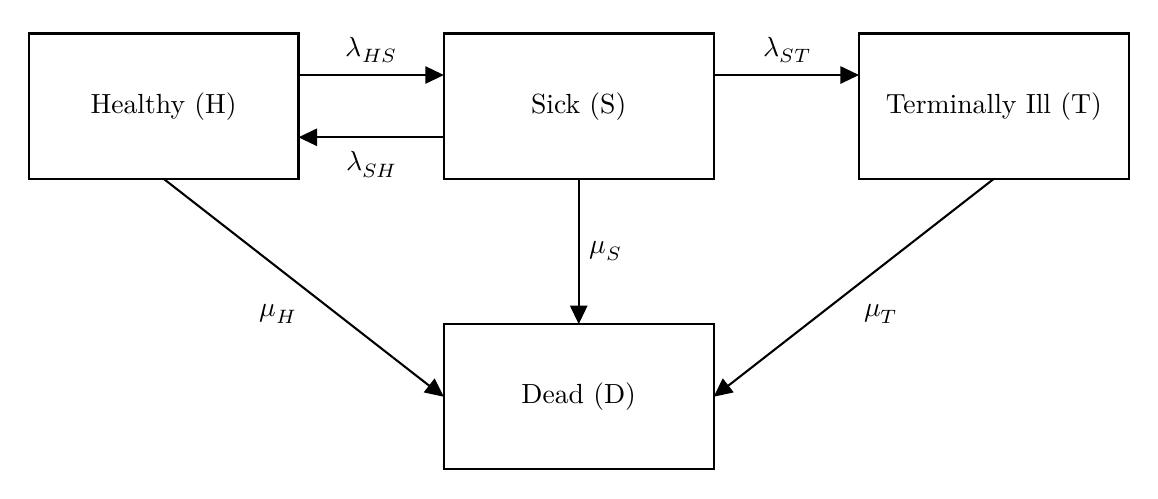
\begin{tikzpicture}[x=0.75pt,y=0.75pt,yscale=-1,xscale=1]

% --- TOP ROW: HEALTHY (H), SICK (S), TERMINALLY ILL (T) ---

% Shape: Rectangle (Healthy - H)
\draw   (20,40) -- (150,40) -- (150,110) -- (20,110) -- cycle ;
% Text Node (H)
\draw (85,75) node  [align=center] {{\fontfamily{ptm}\selectfont Healthy (H)}};

% Shape: Rectangle (Sick - S)
\draw   (220,40) -- (350,40) -- (350,110) -- (220,110) -- cycle ;
% Text Node (S)
\draw (285,75) node  [align=center] {{\fontfamily{ptm}\selectfont Sick (S)}};

% Shape: Rectangle (Terminally Ill - T)
\draw   (420,40) -- (550,40) -- (550,110) -- (420,110) -- cycle ;
% Text Node (T)
\draw (485,75) node  [align=center] {{\fontfamily{ptm}\selectfont Terminally Ill (T)}};


% --- SECOND ROW: DEAD (D) ---

% Shape: Rectangle (Dead - D)
\draw   (220,180) -- (350,180) -- (350,250) -- (220,250) -- cycle ;
% Text Node (D)
\draw (285,215) node  [align=center] {{\fontfamily{ptm}\selectfont Dead (D)}};


% --- HORIZONTAL TRANSITIONS (TOP ROW) ---

% Arrow: H -> S
\draw    (150,60) -- (218,60) ;
\draw [shift={(220,60)}, rotate = 180] [fill={rgb, 255:red, 0; green, 0; blue, 0 }  ][line width=0.75]  [draw opacity=0] (8.93,-4.29) -- (0,0) -- (8.93,4.29) -- cycle    ;
\draw (185,48) node   {$\lambda_{HS}$};

% Arrow: S -> H (Recovery)
\draw    (220,90) -- (152,90) ;
\draw [shift={(150,90)}, rotate = 0] [fill={rgb, 255:red, 0; green, 0; blue, 0 }  ][line width=0.75]  [draw opacity=0] (8.93,-4.29) -- (0,0) -- (8.93,4.29) -- cycle    ;
\draw (185,103) node   {$\lambda_{SH}$};

% Arrow: S -> T
\draw    (350,60) -- (418,60) ;
\draw [shift={(420,60)}, rotate = 180] [fill={rgb, 255:red, 0; green, 0; blue, 0 }  ][line width=0.75]  [draw opacity=0] (8.93,-4.29) -- (0,0) -- (8.93,4.29) -- cycle    ;
\draw (385,48) node   {$\lambda_{ST}$};

% Arrow: T -> S (Optional: remove if T -> S recovery is not allowed)
%\draw    (420,90) -- (352,90) ;
%\draw [shift={(350,90)}, rotate = 0] [fill={rgb, 255:red, %0; green, 0; blue, 0 }  ][line width=0.75]  [draw %opacity=0] (8.93,-4.29) -- (0,0) -- (8.93,4.29) -- cycle    ;
%\draw (385,103) node   {$\lambda_{TS}$};


% --- TRANSITIONS TO DEAD (D) ---

% Arrow: H -> D
\draw    (85,110) -- (218.2,213.77) ;
\draw [shift={(220,215)}, rotate = 217.87] [fill={rgb, 255:red, 0; green, 0; blue, 0 }  ][line width=0.75]  [draw opacity=0] (8.93,-4.29) -- (0,0) -- (8.93,4.29) -- cycle    ;
\draw (140,175) node   {$\mu_{H}$};

% Arrow: S -> D
\draw    (285,110) -- (285,178) ;
\draw [shift={(285,180)}, rotate = 270] [fill={rgb, 255:red, 0; green, 0; blue, 0 }  ][line width=0.75]  [draw opacity=0] (8.93,-4.29) -- (0,0) -- (8.93,4.29) -- cycle    ;
\draw (298,145) node   {$\mu_{S}$};

% Arrow: T -> D
\draw    (485,110) -- (351.8,213.77) ;
\draw [shift={(350,215)}, rotate = 322.13] [fill={rgb, 255:red, 0; green, 0; blue, 0 }  ][line width=0.75]  [draw opacity=0] (8.93,-4.29) -- (0,0) -- (8.93,4.29) -- cycle    ;
\draw (430,175) node   {$\mu_{T}$};

\end{tikzpicture}
\end{center}
\end{frame}

\begin{frame}{Solution: Worked Example}
\protect\phantomsection\label{solution-worked-example}
\end{frame}

\section{The Jump Chain}\label{the-jump-chain}

\begin{frame}{From Holding Times to the Jump Chain}
\protect\phantomsection\label{from-holding-times-to-the-jump-chain}
A Markov jump process describes two aspects of the evolution of a
system:

\begin{itemize}
\tightlist
\item
  \textbf{Timing:} how long the process remains in its current state
  before the next transition.
\item
  \textbf{Destination:} the state to which the process moves when a
  transition occurs.
\end{itemize}

Suppose the process is currently in state \(i\). The total rate of
leaving this state is

\[
\lambda_i=-q_{ii}=\sum_{j\neq i}q_{ij}.
\]

The holding time in state \(i\) is exponentially distributed with
parameter \(\lambda_i\).
\end{frame}

\begin{frame}{From Holding Times to the Jump Chain}
\protect\phantomsection\label{from-holding-times-to-the-jump-chain-1}
When the process leaves state \(i\), it moves to state \(j\) with
probability

\[
\frac{q_{ij}}{\lambda_i},\qquad j\neq i.
\]

The next result shows that, conditional on the current state, the
holding time and the destination of the next transition are independent.
\end{frame}

\begin{frame}{Distribution of the Next State}
\protect\phantomsection\label{distribution-of-the-next-state}
\textbf{Theorem:} Given that a time-homogeneous Markov jump process is
currently in state \(i\), where \(\lambda_i>0\), the probability that it
moves to state \(j\) when it leaves state \(i\) is

\[
\boxed{
\Pr(X(T_1)=j\mid X(0)=i)
=\frac{q_{ij}}{-q_{ii}},
\qquad j\neq i,
}
\]

where \(T_1\) is the time of the first jump.

Furthermore, the destination of the next transition is independent of
the first holding time, conditional on \(X(0)=i\).

Thus, the first holding time determines \textbf{when} the next
transition occurs, while the transition probabilities determine
\textbf{where} the process moves.
\end{frame}

\begin{frame}{Independence of the Holding Time and the Destination}
\protect\phantomsection\label{independence-of-the-holding-time-and-the-destination}
The independence result can be seen from the joint probability density.

For a small interval \(dt\), the probability that the process remains in
state \(i\) until time \(t\) and then moves to state \(j\) is
approximately

\[
\Pr(T_1\in[t,t+dt),\,X(T_1)=j\mid X(0)=i)
=
e^{-\lambda_i t}q_{ij}\,dt.
\]

Since

\[
e^{-\lambda_i t}q_{ij}
=
\underbrace{\lambda_i e^{-\lambda_i t}}_{\text{Holding-time density}}
\underbrace{\frac{q_{ij}}{\lambda_i}}_{\text{Jump probability}},
\]

the joint density factors into the product of the holding-time density
and the jump probability.

Therefore, conditional on the current state, the holding time and the
destination of the next jump are independent.
\end{frame}

\begin{frame}{Definition of the Jump Chain}
\protect\phantomsection\label{definition-of-the-jump-chain}
Consider a time-homogeneous Markov jump process \(\{X(t),t\geq 0\}\).

Let

\[
T_0=0
\]

and, for \(n\geq 1\), let \(T_n\) denote the time of the \(n\)th jump,
where a jump is a transition to a different state.

Define

\[
X_n^*=X(T_n),\qquad n\geq 0.
\]
\end{frame}

\begin{frame}{Definition of the Jump Chain}
\protect\phantomsection\label{definition-of-the-jump-chain-1}
The sequence

\[
X_0^*,X_1^*,X_2^*,\ldots
\]

records the states visited by the process at successive jump times.

This sequence forms a discrete-time Markov chain, called the
\textbf{jump chain} or \textbf{embedded Markov chain}.

Unlike the original continuous-time process, the jump chain records only
the sequence of states visited and ignores the time spent in each state.
\end{frame}

\begin{frame}{Transition Matrix of the Jump Chain}
\protect\phantomsection\label{transition-matrix-of-the-jump-chain}
Let \(P^*=(p_{ij}^*)\) denote the transition matrix of the jump chain.

If \(q_{ii}<0\), the probability of moving from state \(i\) to a
different state \(j\) at the next jump is

\[
\boxed{
p_{ij}^*=\frac{q_{ij}}{-q_{ii}},
\qquad j\neq i,
}
\]

with \(p_{ii}^*=0.\)

If \(q_{ii}=0\), state \(i\) is absorbing. We define

\[
p_{ii}^*=1,
\qquad
p_{ij}^*=0,\quad j\neq i.
\]

Thus, every row of \(P^*\) sums to one.

The jump chain describes the sequence of states visited by the
continuous-time process.
\end{frame}

\begin{frame}{Relationship Between the Markov Jump Process and Its Jump
Chain}
\protect\phantomsection\label{relationship-between-the-markov-jump-process-and-its-jump-chain}
The Markov jump process and its jump chain describe the same sequence of
state changes, but in different ways.

{\def\LTcaptype{none} % do not increment counter
\begin{longtable}[]{@{}
  >{\raggedright\arraybackslash}p{(\linewidth - 2\tabcolsep) * \real{0.5000}}
  >{\raggedright\arraybackslash}p{(\linewidth - 2\tabcolsep) * \real{0.5000}}@{}}
\toprule\noalign{}
\begin{minipage}[b]{\linewidth}\raggedright
Markov jump process
\end{minipage} & \begin{minipage}[b]{\linewidth}\raggedright
Jump chain
\end{minipage} \\
\midrule\noalign{}
\endhead
Continuous-time process & Discrete-time Markov chain \\
Records the time spent in each state & Ignores the holding times \\
Uses transition rates \(q_{ij}\) & Uses transition probabilities
\(p_{ij}^*\) \\
Describes when and where transitions occur & Describes only the sequence
of states visited \\
\bottomrule\noalign{}
\end{longtable}
}

The jump chain is useful for questions concerning the order in which
states are visited.

For example:

\begin{itemize}
\tightlist
\item
  What is the probability of reaching state D before state H?
\item
  What is the probability of visiting a particular state before reaching
  an absorbing state?
\item
  What is the probability of eventually reaching a specified state?
\end{itemize}

These questions can be answered using the theory of discrete-time Markov
chains.
\end{frame}

\begin{frame}{Worked Example: The Jump Chain of a Four-State Health
Model}
\protect\phantomsection\label{worked-example-the-jump-chain-of-a-four-state-health-model}
Consider the Health--Sickness--Terminally Ill--Death (HSTD) model
introduced earlier.

Using the given transition rates:

\begin{enumerate}
\item
  Write down the generator matrix \(Q\) for the four-state
  continuous-time Markov model.
\item
  Obtain the transition matrix \(P^*\) of the associated jump chain,
  using

  \[
  p_{ij}^*=\frac{q_{ij}}{-q_{ii}},
  \qquad i\neq j.
  \]
\item
  (Direct transition probability) Calculate the probability that an
  individual in state S moves directly to state D when leaving state S.
\item
  (Hitting probability) Determine the probability that a life starting
  in the Sick state reaches Death without first returning to the Healthy
  state.
\end{enumerate}
\end{frame}

\begin{frame}{Worked Example: The Jump Chain of a Four-State Health
Model}
\protect\phantomsection\label{worked-example-the-jump-chain-of-a-four-state-health-model-1}
\textbf{Key distinction:} The direct transition probability considers
only the next jump, whereas the hitting probability considers all paths
that reach \(D\) before \(H\).

\textbf{Hint for Question 4}

Let \(h_i\) denote the probability of reaching Death before Healthy,
starting from state \(i\).

The boundary conditions are

\[
h_H=0,\qquad h_D=1.
\]

For the other states, use the first-step equations

\[
h_i=\sum_j p_{ij}^*h_j.
\]

Solve the resulting equations to obtain \(h_S\).
\end{frame}

\begin{frame}{Solution: Worked Example}
\protect\phantomsection\label{solution-worked-example-1}
\end{frame}

\section{Expected Time to Reach a Given
State}\label{expected-time-to-reach-a-given-state}

\begin{frame}{Expected Time to Reach a Target State}
\protect\phantomsection\label{expected-time-to-reach-a-target-state}
Suppose we are interested in the expected time required for a Markov
jump process to reach a specified target state \(k\).

For example, in an actuarial model, we may wish to calculate:

\begin{itemize}
\tightlist
\item
  the expected time until a policyholder dies;
\item
  the expected time until a policyholder becomes terminally ill;
\item
  the expected time until a company reaches default.
\end{itemize}

Let \(m_i\) denote the expected time to reach state \(k\), given that
the process starts in state \(i\).

By definition,

\[
m_k=0,
\]

since the process has already reached the target state when it starts in
state \(k\).
\end{frame}

\begin{frame}{Recursive Formula for Expected Hitting Times}
\protect\phantomsection\label{recursive-formula-for-expected-hitting-times}
Suppose the process starts in a state \(i\neq k\), with total transition
rate

\[
\lambda_i=-q_{ii}>0.
\]

The process first spends a holding time in state \(i\), whose expected
value is

\[
\frac{1}{\lambda_i}.
\]

It then moves to another state \(j\) with probability

\[
p_{ij}^*=\frac{q_{ij}}{\lambda_i}.
\]

If the process moves to state \(j\), the expected additional time
required to reach state \(k\) is \(m_j\).
\end{frame}

\begin{frame}{Recursive Formula for Expected Hitting Times}
\protect\phantomsection\label{recursive-formula-for-expected-hitting-times-1}
Using first-step analysis,

\[
m_i
=
\frac{1}{\lambda_i}
+
\sum_{j\neq i}p_{ij}^*m_j.
\]

Therefore,

\[
\boxed{
m_i
=
\frac{1}{\lambda_i}
+
\sum_{\substack{j\neq i\\j\neq k}}
\frac{q_{ij}}{\lambda_i}m_j,
\qquad i\neq k.
}
\]

The target-state term is omitted because \(m_k=0\).
\end{frame}

\begin{frame}{Interpreting the Recursive Formula}
\protect\phantomsection\label{interpreting-the-recursive-formula}
The expected time to reach state \(k\) consists of two parts:

\[
\underbrace{m_i}_{\text{Expected time to reach }k}
=
\underbrace{\frac{1}{\lambda_i}}_{\text{Expected holding time in }i}
+
\underbrace{\sum_{j\neq i}p_{ij}^*m_j}_{\text{Expected remaining time after the next jump}}.
\]

The first term is the expected time spent in the current state.

The second term is the expected time remaining after the process leaves
the current state, averaged over all possible destination states.

The recursive equations are solved simultaneously for all non-target
states.

If the target state cannot be reached with probability one, the expected
hitting time may be infinite. A non-target absorbing state, for example,
gives an infinite expected time to reach \(k\).
\end{frame}

\begin{frame}{Worked Example: Expected Future Lifetime in the HSTD
Model}
\protect\phantomsection\label{worked-example-expected-future-lifetime-in-the-hstd-model}
Return to the four-state Health--Sickness--Terminally Ill--Death model.

Suppose the target state is Death (D), and let

\begin{itemize}
\tightlist
\item
  \(m_H\) denote the expected future lifetime of a healthy life;
\item
  \(m_S\) denote the expected future lifetime of a sick life;
\item
  \(m_T\) denote the expected future lifetime of a terminally ill life.
\end{itemize}

\textbf{Questions}

\begin{enumerate}
\item
  Write down the recursive equations for \(m_H\), \(m_S\) and \(m_T\),
  using the expected holding times and transition probabilities of the
  associated jump chain.
\item
  Solve the resulting system of simultaneous equations to determine the
  expected future lifetime of an individual who is initially in state H.
\end{enumerate}
\end{frame}

\begin{frame}{(Brief) Solution to Worked Example: Expected Future
Lifetime in the HSTD Model}
\protect\phantomsection\label{brief-solution-to-worked-example-expected-future-lifetime-in-the-hstd-model}
Since Death is the target state,

\[
m_D=0.
\]

For each non-absorbing state, apply the recursive formula:

\[
m_i
=
\frac{1}{\lambda_i}
+
\sum_{j\neq i}p_{ij}^*m_j.
\]

This gives a system of three simultaneous equations.

Solving the system gives the expected future lifetime of a healthy life,
\(m_H\).

\textbf{The numerical solution depends on the transition rates specified
in the HSTD model.}
\end{frame}

\section{Observing a Markov Jump Process at an Arbitrary
Time}\label{observing-a-markov-jump-process-at-an-arbitrary-time}

\begin{frame}{Residual Holding Time}
\protect\phantomsection\label{residual-holding-time}
So far, we have considered the first holding time when the initial state
\(X(0)\) is given.

We can extend this idea by observing the process at an arbitrary time
\(s>0\) and considering the additional time until its next transition.

Suppose that \(X(s)=i\). The \textbf{residual holding time} is defined
as

\[
T_s=\inf\{t>0:X(s+t)\neq X(s)\}.
\]

For a time-homogeneous Markov jump process,

\[
\boxed{
T_s\mid X(s)=i\sim\operatorname{Exp}(\lambda_i),
}
\]

where

\[
\lambda_i=\sum_{j\neq i}q_{ij}=-q_{ii}.
\]
\end{frame}

\begin{frame}{Residual Holding Time}
\protect\phantomsection\label{residual-holding-time-1}
Consequently,

\[
\Pr(T_s>t\mid X(s)=i)=e^{-\lambda_i t}.
\]

The remaining time in state \(i\) has the same exponential distribution,
regardless of how long the process has already spent in that state.
\end{frame}

\begin{frame}{Distribution of the Next State at an Arbitrary Observation
Time}
\protect\phantomsection\label{distribution-of-the-next-state-at-an-arbitrary-observation-time}
Suppose that the process is observed in state \(i\) at time \(s\), where
\(\lambda_i>0\).

The probability that the next transition is to state \(j\) is

\[
\boxed{
\Pr(X(s+T_s)=j\mid X(s)=i)
=\frac{q_{ij}}{\lambda_i},
\qquad j\neq i.
}
\]

Thus, the probability of moving to a particular state at the next jump
does not depend on the observation time \(s\).

Furthermore, conditional on \(X(s)=i\), the destination of the next
transition is independent of the residual holding time \(T_s\).
\end{frame}

\begin{frame}{Connection with the Results at Time 0}
\protect\phantomsection\label{connection-with-the-results-at-time-0}
The results obtained at time 0 extend directly to an arbitrary
observation time \(s>0\).

In particular, conditional on the current state being \(i\):

\begin{itemize}
\item
  The first holding time and the residual holding time have the same
  exponential distribution:

  \[
  T_0\sim\operatorname{Exp}(\lambda_i),
  \qquad
  T_s\sim\operatorname{Exp}(\lambda_i).
  \]
\item
  The probability of moving to state \(j\) at the next jump is the same:

  \[
  \Pr(\text{next state}=j)
  =\frac{q_{ij}}{\lambda_i},
  \qquad j\neq i.
  \]
\item
  In both cases, the holding time and the destination of the next
  transition are conditionally independent.
\end{itemize}
\end{frame}

\begin{frame}{Connection with the Results at Time 0}
\protect\phantomsection\label{connection-with-the-results-at-time-0-1}
Therefore, the same distributions describe \textbf{when} the next
transition occurs and \textbf{where} the process moves, whether it is
observed at time 0 or at a later time.

These results provide the basis for describing the sequence of states
visited at successive jumps, which leads to the definition of the
\textbf{jump chain}.
\end{frame}




\end{document}
